% Estas slides tienen que abrirse con el programa pdfpc que soporta videos embebidos. Para los videos se requiere ubuntu-restricted-extras. El comando es: pdfpc -g slides.pdf

% compress: Encabezado muestra solo la section actual
\documentclass[compress]{beamer}
\mode<presentation>

\usetheme{Copenhagen}
\useoutertheme{taihu}
\useinnertheme{rectangles}

% Itemize configuration
\setbeamertemplate{itemize item}[rectangle]
\setbeamertemplate{itemize subitem}[circle]
\setbeamertemplate{itemize subsubitem}[triangle]

\setbeamertemplate{navigation symbols}{} % Remover símbolos de navegación
\usefonttheme[onlymath]{serif} % Símbolos matemáticos en Serif

\setbeamertemplate{blocks}[rounded] % Block corners rounded
\setbeamercolor{block body}{bg=blue!12,fg=black} % Color of blocks

\usepackage{pdfpc-commands} % pdfpc movie commands
\usepackage[utf8]{inputenc}
\usepackage[spanish]{babel}
\usepackage[binary-units=true]{siunitx} % Para manejar las unidades
\usepackage{multirow}
\usepackage{multimedia}
\usepackage{graphicx}
\usepackage{xcolor}
\usepackage{booktabs} % \toprule

% Elimina la palabra 'Figura' del caption
\usepackage[caption=false]{subfig}
\setbeamertemplate{caption}{\raggedright\insertcaption\par}
\captionsetup[subfigure]{labelformat=empty} % Remover índice del caption de la subfigura

\usepackage{import} % Para el comando import (se usa para pdf_tex)

% Para notas personales en el pdfpc
\usepackage{pdfpcnotes}

\AtBeginSection[]
{
   \begin{frame}
       \frametitle{Índice}
       \tableofcontents[currentsection]
   \end{frame}
}

\usepackage{amsmath}
\usepackage{amssymb}
\usepackage{amsopn}

% math
\renewcommand{\vec}[1]{\boldsymbol{\mathbf{#1}}}
\newcommand{\norm}[1]{\left\lVert#1\right\rVert}

% Declare arg max and arg min functionss
\DeclareMathOperator*{\argmax}{arg\,max}
\DeclareMathOperator*{\argmin}{arg\,min}

% Homogeneous decoration function
\newcommand{\homo}[1]{\dot{#1}}

% Declare projection as math function
\DeclareMathOperator{\proj}{proj}
\DeclareMathOperator{\disp}{disp}
\newcommand{\worldCoordSystem}{\mathrm{w}}
\newcommand{\cameraCoordSystem}{\mathrm{c}}
\newcommand{\point}{\vec{x}}
\newcommand{\worldPoint}{\point^{\mathrm{w}}}
\newcommand{\homoWorldPoint}{\homo{\point}^{\mathrm{w}}}
\newcommand{\cameraPoint}{\point^{\mathrm{c}}}
\newcommand{\hatCameraPoint}{\hat{\point}^{\mathrm{c}}}
\newcommand{\homoCameraPoint}{\homo{\point}^{\mathrm{c}}}
\newcommand{\measurement}{\vec{z}}
\newcommand{\prediction}{\hat{\vec{z}}}
\newcommand{\imagePoint}{\vec{u}}
\newcommand{\seMatrix}{\vec{E}}
\newcommand{\rotation}{\vec{R}}
\newcommand{\translation}{\vec{t}}
\newcommand{\intrinsicMatrix}{\vec{K}}
\newcommand{\principalPoint}{\vec{c}}
\newcommand{\reprojectionError}{u}
\newcommand{\projectionMatrix}{\vec{P}}
\newcommand{\cameraCenter}{\vec{o}}


% Dense Map
\newcommand{\current}{\mathrm{current}}
\newcommand{\previous}{\mathrm{previous}}
\newcommand{\fusion}{\mathrm{fusion}}
\newcommand{\inverseDepth}{\rho}
\newcommand{\plane}{\boldsymbol{\pi}}
\newcommand{\reference}{ref}


% scaled operators and letters to fancy view
\newcommand{\sminus}{\scalebox{0.5}[1.0]{$-$}}
\newcommand{\splus}{\scalebox{0.6}[0.6]{$+$}}
\newcommand{\curr}{c}
\newcommand{\sind}[1]{\scalebox{0.6}[0.6]{$#1$}}
\newcommand{\ind}[1]{\scalebox{0.7}[0.7]{$#1$}}

\newcommand{\keyframe}{\vec{K}}
\newcommand{\pointCloud}{\mathcal P}
\newcommand{\groundTruth}[1]{{#1}^{*}}

\newcommand{\update}[1]{\hat{#1}}

\newcommand{\position}{\vec{p}}
\newcommand{\map}{M}

\newcommand{\baseline}{b}
\newcommand{\focalDistance}{f}
\newcommand{\disparityMap}{\mathcal D}
\newcommand{\camera}{c}
\newcommand{\ray}{n}


\setbeamerfont{normal text}{size*={10}{10}}
\AtBeginDocument{\usebeamerfont{normal text}}

\title{Mapeo denso en tiempo real sobre sistemas SLAM basados en visión estéreo}
\author{Ariel D'Alessandro}
\institute{Director: Taihú Pire. Co-Director: Rodrigo Baravalle. \\ \vspace{0.5cm} Tesina de Grado \\ Licenciatura en Ciencias de la Computación \\ FCEIA - UNR}
\titlegraphic{
\includegraphics[width=0.14\textwidth]{images/logo-unr.png}}
\date{\scriptsize{22 de diciembre de 2017}}

\begin{document}

\frame{\titlepage}

\begin{frame}
\frametitle{Índice}
\tableofcontents
\end{frame}


\section{Introducción}


\subsection{Presentación}


\begin{frame}
\frametitle{Motivación}

\begin{block}{Objetivo a desarrollar}
Método de reconstrucción 3D o mapeo denso en tiempo real sobre sistemas de localización y mapeo simultáneo (SLAM) basado en visión estéreo.
\end{block}

\end{frame}


\begin{frame}
\frametitle{Reconstrucción 3D}

\pnote{* Reconstrucción 3D: Proceso mediante el cual se captura y representa la forma y apariencia de entornos u objetos presentes en la realidad. Diseño asistido por computadora, imágenes médicas, realidad virtual y aumentada, robótica movil, entre otros.}

\pnote{* Uno de los principales problemas presentes en aplicaciones relativas a robots autónomos móviles consiste en el planeamiento de una trayectoria segura hacia determinados objetivos, mientras el robot se desplaza a través de un entorno potencialmente desconocido.}

\pnote{* Para esto, resulta necesario contar con una representación del ambiente que se está transitando (mapa) y la ubicación del robot dentro del mismo (SLAM - slide siguiente).}

\pnote{* El mapa debe ser suficientemente detallado (denso) para que el robot pueda realizar un planeamiento seguro, evitando posibles obstáculos.}

\begin{figure}[!htb]
	\centering
	\subfloat[]{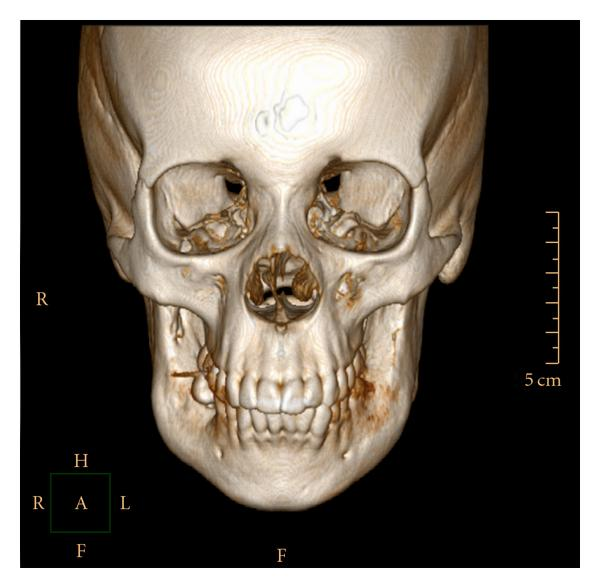
\includegraphics[width=0.30\columnwidth]{./introduction/3d-skull.jpg}}%
	\hfill
	\subfloat[]{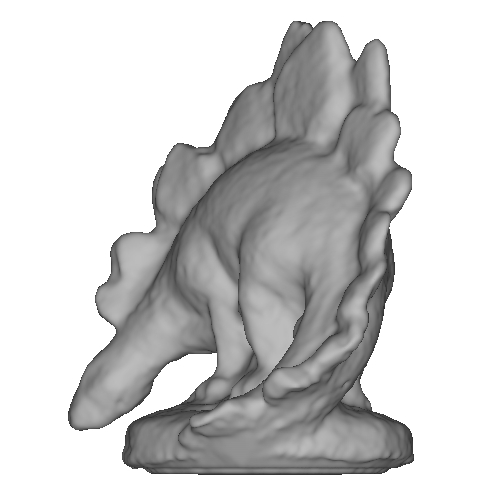
\includegraphics[width=0.30\columnwidth]{./introduction/3d-dinosaur.jpg}}%
	\hfill
	\centering
	\subfloat[]{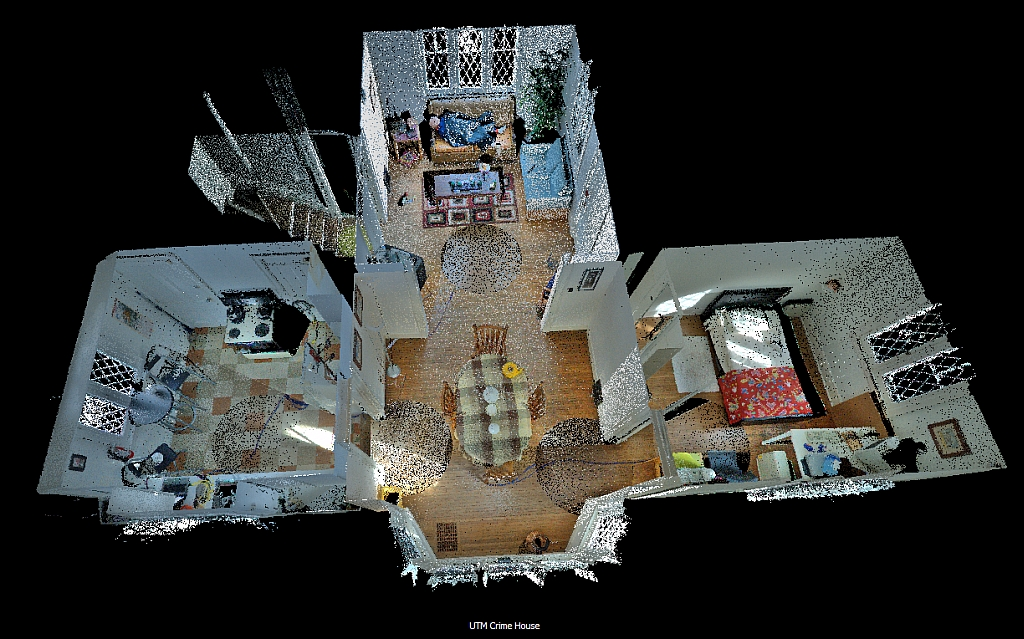
\includegraphics[width=0.40\columnwidth]{./introduction/3d-indoor.jpg}}%
	\hfill
	\\
	\centering
	\subfloat[]{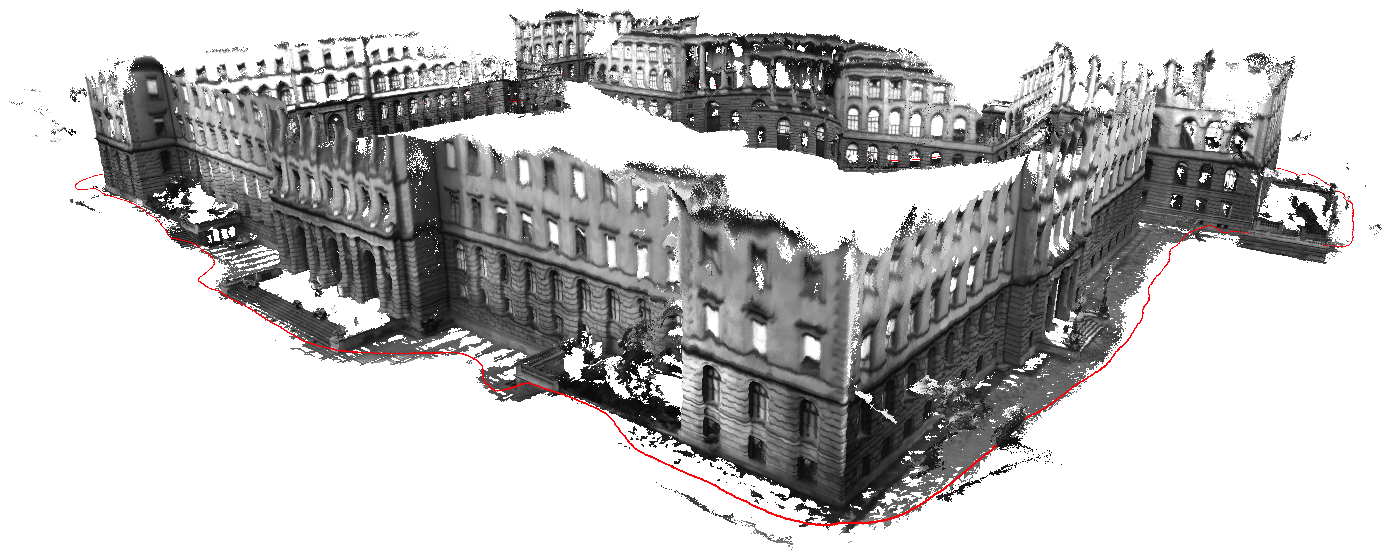
\includegraphics[width=0.70\columnwidth]{./introduction/3d-building.png}}%
	\hfill
\end{figure}

\end{frame}


\subsection{SLAM}


\begin{frame}
\frametitle{SLAM - Simultaneous Localisation and Mapping}

\pnote{* A partir de la detección y seguimiento de marcas naturales del ambiente (landmarks), los sistemas de SLAM pueden estimar tanto la posición del robot como la ubicación de estas marcas en el entorno. El mapa es construído incrementalmente con las posiciones estimadas de dichas marcas, las cuales son ajustadas a lo largo de la trayectoria a medida que son observadas.}

\begin{itemize}
\item Construir incrementalmente un mapa del entorno.
\item Determinar su posición y orientación en el mismo.
\end{itemize}

\begin{figure}[!htb]
	\centering
	\subfloat[]{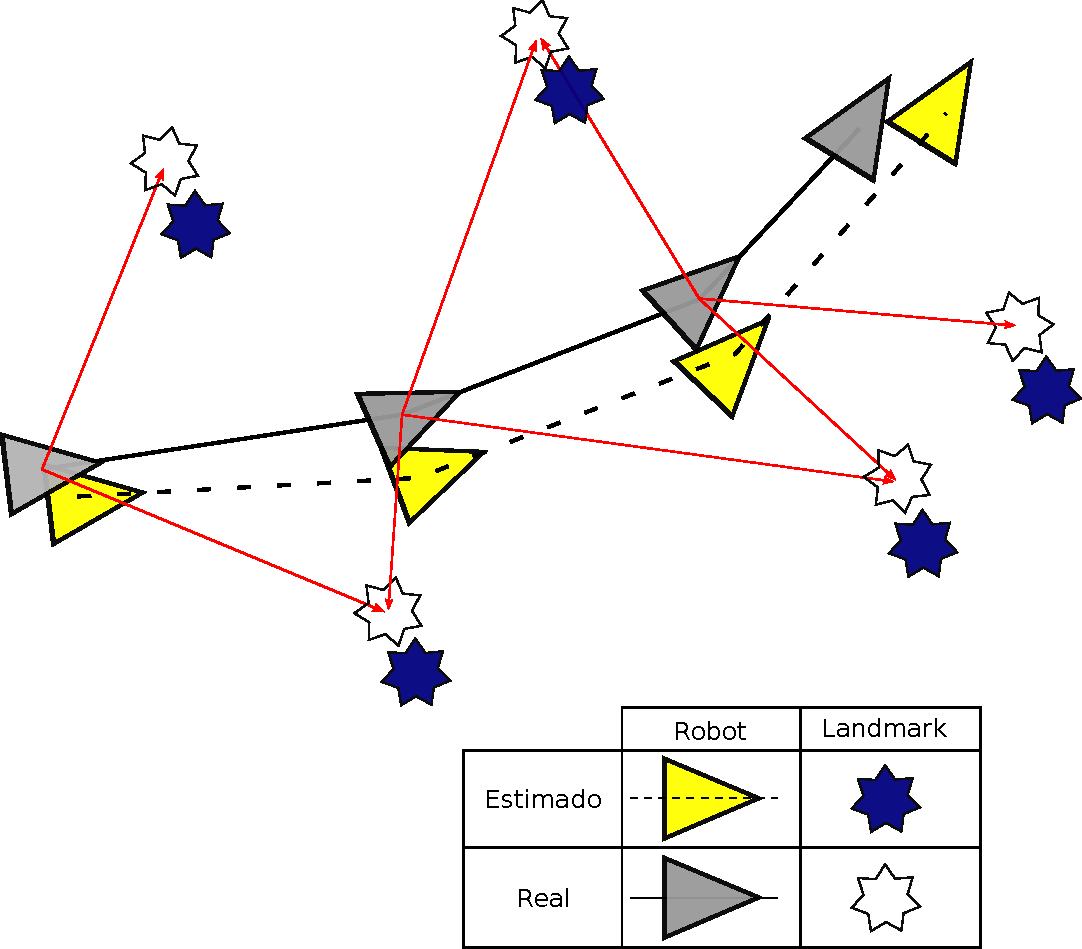
\includegraphics[width=0.50\columnwidth]{./introduction/slam-landmarks.pdf}}%
	\hfill
\end{figure}

\end{frame}


\subsection{SLAM Visual}


\begin{frame}
\frametitle{SLAM Visual - Cámaras}

\pnote{* Cámaras: rica información de la escena. Ventajas: bajo costo, menor consumo energético en comparación con otros sensores, como lásers, portabilidad y alta disponibilidad en dispositivos móviles. Son sensores pasivos por lo que no interferen con otros sensores y pueden utilizarse en entornos interiores, donde el uso de GPS puede verse imposibilitado. Asímismo, son menos restrictivos que los encoders, los cuales se encuentran limitados a robots terrestres y resultan imprecisos en terrenos irregulares.}

\begin{itemize}
\item Bajo costo.
\item Bajo consumo energético.
\item Alta disponibilidad en dispositivos móviles.
\item Sensores pasivos.
\item Apto entornos interiores.
\item Apto terrenos irregulares.
\end{itemize}

\end{frame}


\begin{frame}
\frametitle{SLAM Visual - Cámaras estéreo}

\pnote{* Cámaras estéreo: Existen dos enfoques predominantes en los sistemas de SLAM basados en cámaras, denominados monocular y estéreo. Los sistemas de SLAM visual estéreo proveen información sobre la profundidad de los píxeles mediante una única observación, lo cual requiere mayor número de cómputos en el caso monocular.}

\begin{figure}[!htb]
	\centering
	\subfloat[]{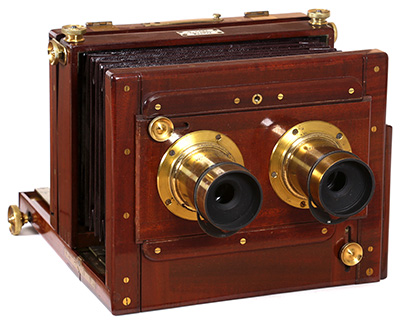
\includegraphics[width=0.45\columnwidth]{./introduction/camera-stereo-old.jpg}}%
	\hfill
	\centering
	\subfloat[]{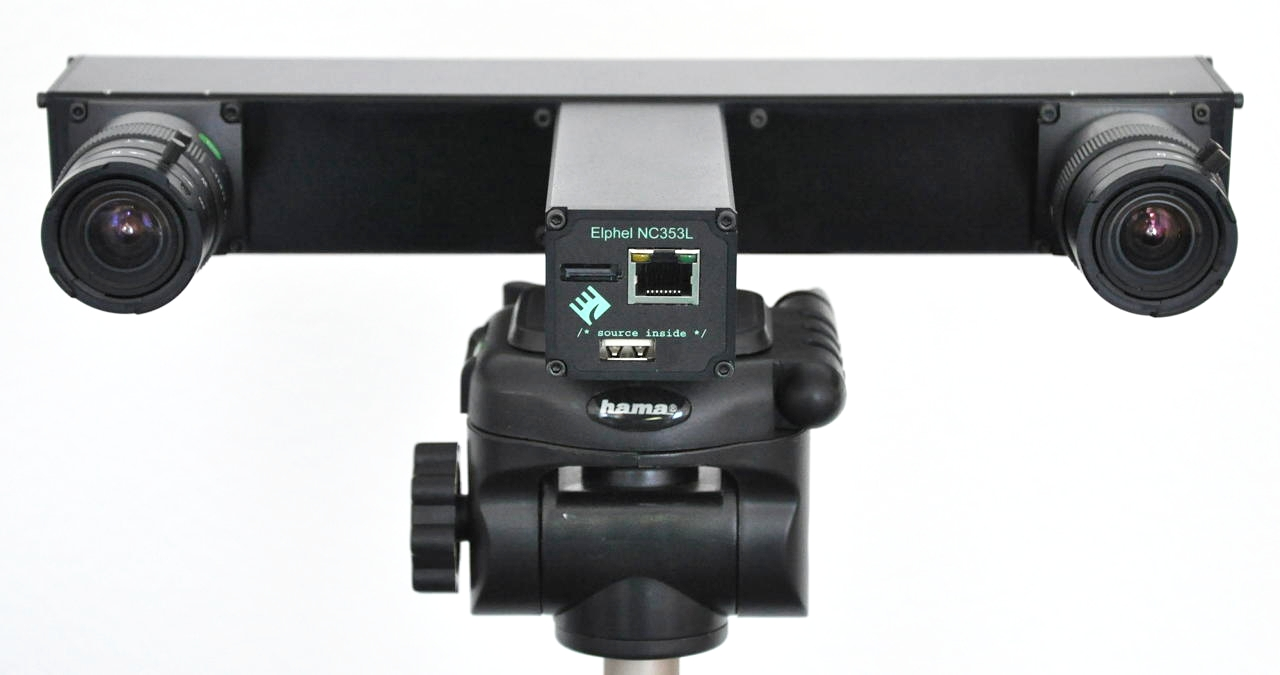
\includegraphics[width=0.45\columnwidth]{./introduction/camera-stereo-new.jpg}}%
	\hfill
\end{figure}

\end{frame}


\section{Conceptos básicos}


\subsection{Cámaras}


\begin{frame}
\frametitle{Modelo de cámara}

\begin{block}{Definición - Cámara}
Una cámara es definida matemáticamente como una correspondencia entre el mundo 3D y una imagen 2D. Es decir, un mapeo entre puntos del mundo 3D $\point$ y puntos de la imagen $\imagePoint$:
\begin{equation}
\point=\begin{bmatrix}x\\
y\\
z
\end{bmatrix}\longmapsto
\imagePoint=\begin{bmatrix}u\\
v
\end{bmatrix}
\end{equation}
\end{block}

\end{frame}


\begin{frame}
\frametitle{Modelo de cámara pinhole}

\pnote{* Rayo principal o eje principal de la cámara: rayo que se origina en el centro focal \cameraCenter y es perpendicular al plano de la imagen.}

\pnote{* Punto principal: el punto donde este rayo intersecta al plano de la imagen es denominado.}

\begin{block}{Cámara pinhole}
El punto de la imagen $\imagePoint=\begin{bmatrix}u & v\end{bmatrix}^{\top}$ es determinado como la intersección entre el \emph{plano de la imagen} y el rayo que une el punto del mundo 3D $\point=\begin{bmatrix}x & y & z\end{bmatrix}^{\top}$ con el \emph{centro focal} $\cameraCenter$ de la cámara.
\end{block}

\begin{figure}[!htb]
	\centering
	\subfloat[]{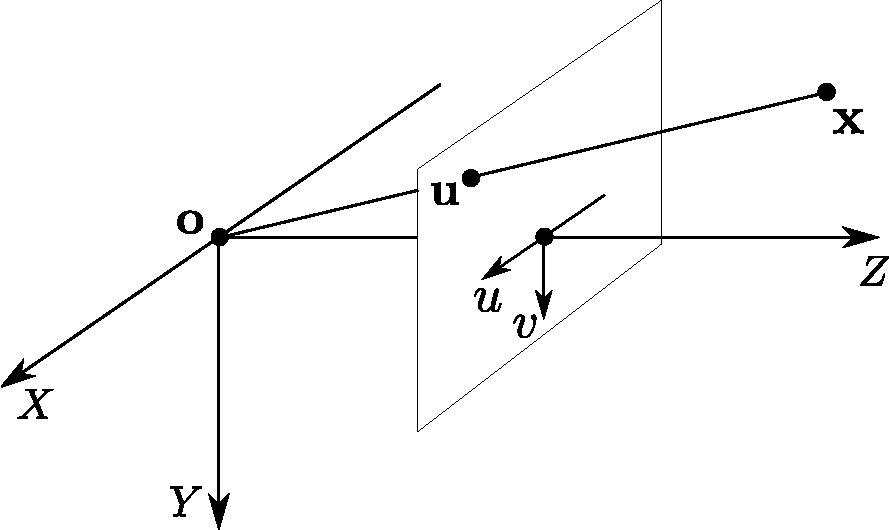
\includegraphics[width=0.5\columnwidth]{./cameras/pinhole_camera_model.pdf}}%
	\hfill
\end{figure}

\end{frame}


\begin{frame}
\frametitle{Modelo de cámara pinhole}

\pnote{* Proyección central: Utilizando la propiedad de semejanza de triángulos, el punto 3D es mapeado al punto en el plano de la imagen.}

\begin{block}{Proyección central}
Asumiendo el centro focal en el origen de coordenadas y el plano de la imagen $Z=f$:

\begin{equation}
\begin{bmatrix}x\\
y\\
z
\end{bmatrix}\longmapsto\begin{bmatrix}fx/z\\
fy/z
\end{bmatrix}
\end{equation}

\end{block}

\begin{figure}[!htb]
	\centering
	\subfloat[]{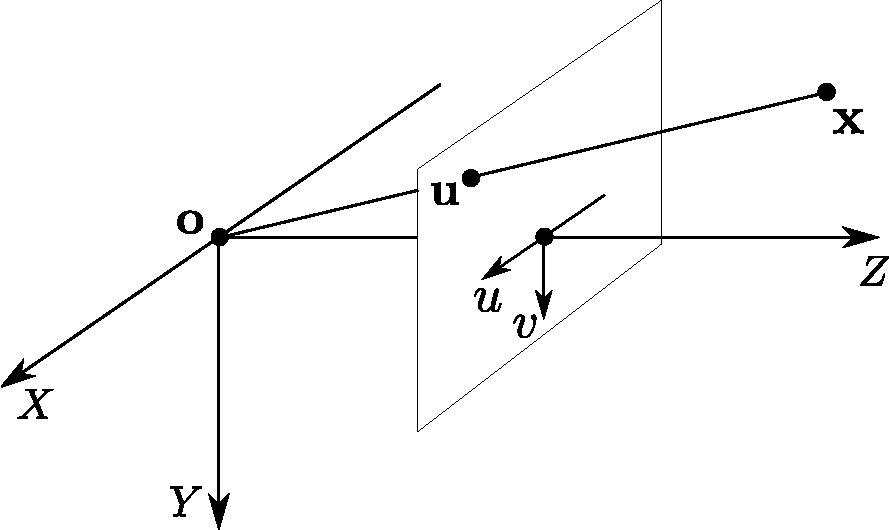
\includegraphics[width=0.5\columnwidth]{./cameras/pinhole_camera_model.pdf}}%
	\hfill
	\centering
	\subfloat[]{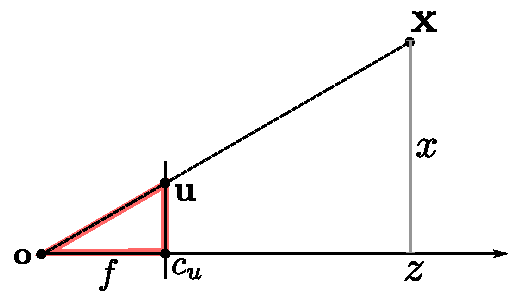
\includegraphics[width=0.5\columnwidth]{./cameras/pinhole_camera_model2.pdf}}%
	\hfill
\end{figure}

\end{frame}


\begin{frame}
\frametitle{Triangulación estéreo}

\pnote{* Sea x = x y z un punto 3D cuyas coordenadas son desconocidas. Conociendo las proyecciones correspondientes, la posición del punto x puede ser derivada.}

\pnote{* Aplicando la propiedad de triángulos semejantes entre el triángulo de línea negra punteada y el triángulo de línea roja en la Figura, la siguiente ecuación puede ser formulada.}

Proyecciones correspondientes $\imagePoint_{l}=\begin{bmatrix}u_{l} & v_{l}\end{bmatrix}$ y $\imagePoint_{r}=\begin{bmatrix}u_{r} & v_{r}\end{bmatrix}$ sobre los planos focales de la imagen izquierda y derecha respectivamente,
la posición del punto $\point$ puede ser derivada.

\begin{equation}
\frac{b}{z}=\frac{(b+u_{r})-u_{l}}{z-f}
\end{equation}

\begin{figure}[!htb]
	\centering
	\subfloat[]{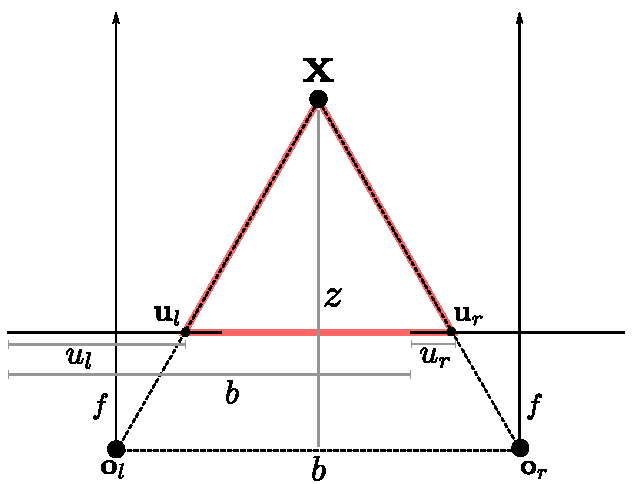
\includegraphics[width=0.5\columnwidth]{./cameras/stereo_triangulation.pdf}}%
	\hfill
	\centering
	\subfloat[]{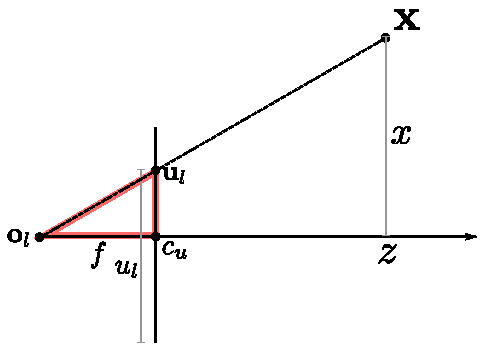
\includegraphics[width=0.5\columnwidth]{./cameras/stereo_triangulation2.pdf}}%
	\hfill
\end{figure}
\end{frame}


\begin{frame}
\frametitle{Triangulación estéreo}

\pnote{* De la misma manera, utilizando propiedad de triángulos semejantes nuevamente sobre la Figura, se obtienen las restantes ecuaciones.}

\begin{equation}
\frac{x}{z}=\frac{u_{l}-c_{u}}{f}\qquad\frac{y}{z}=\frac{v_{l}-c_{v}}{f}
\end{equation}

\begin{equation}
\begin{aligned}x=\frac{(u_{l}-c_{u})z}{f}\;\qquad
y=\frac{(v_{l}-c_{v})z}{f}\;\qquad
z=\frac{bf}{u_{l}-u_{r}}\;
\end{aligned}
\end{equation}

\begin{figure}[!htb]
	\centering
	\subfloat[]{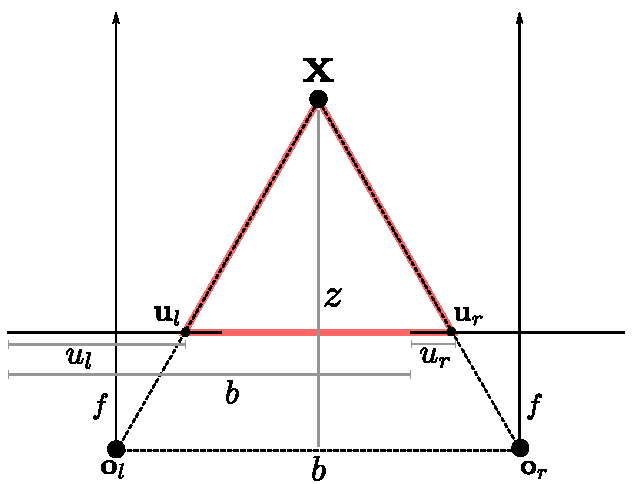
\includegraphics[width=0.5\columnwidth]{./cameras/stereo_triangulation.pdf}}%
	\hfill
	\centering
	\subfloat[]{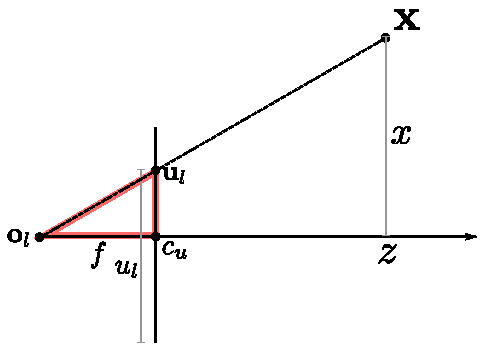
\includegraphics[width=0.5\columnwidth]{./cameras/stereo_triangulation2.pdf}}%
	\hfill
\end{figure}
\end{frame}


\subsection{Disparidad}


\begin{frame}
\frametitle{Disparidad}

\pnote{* Cuando el valor de disparidad $d$ es cercano a $0$, pequeñas diferencias de disparidad producen un gran cambio en la profundidad del punto. En consecuencia, la reconstrucción 3D del ambiente mediante cámaras estéreo es más precisa para puntos cercanos a la cámara.}

\begin{block}{Definición - Disparidad}
La disparidad $d$ es definida como la distancia existente entre las proyecciones de las diferentes cámaras.
\begin{equation}
d=u_{l}-u_{r}=\frac{bf}{z}
\end{equation}
\end{block}

\textbf{Nota}: la profundidad $z$ es inversamente proporcional a la disparidad $d$.

\end{frame}


\section{S-PTAM Denso}


\subsection{S-PTAM}


% Frame ---------------------------------------------------------------------
\begin{frame}
	\frametitle{S-PTAM}
	\begin{figure}[htb]
		\centering
		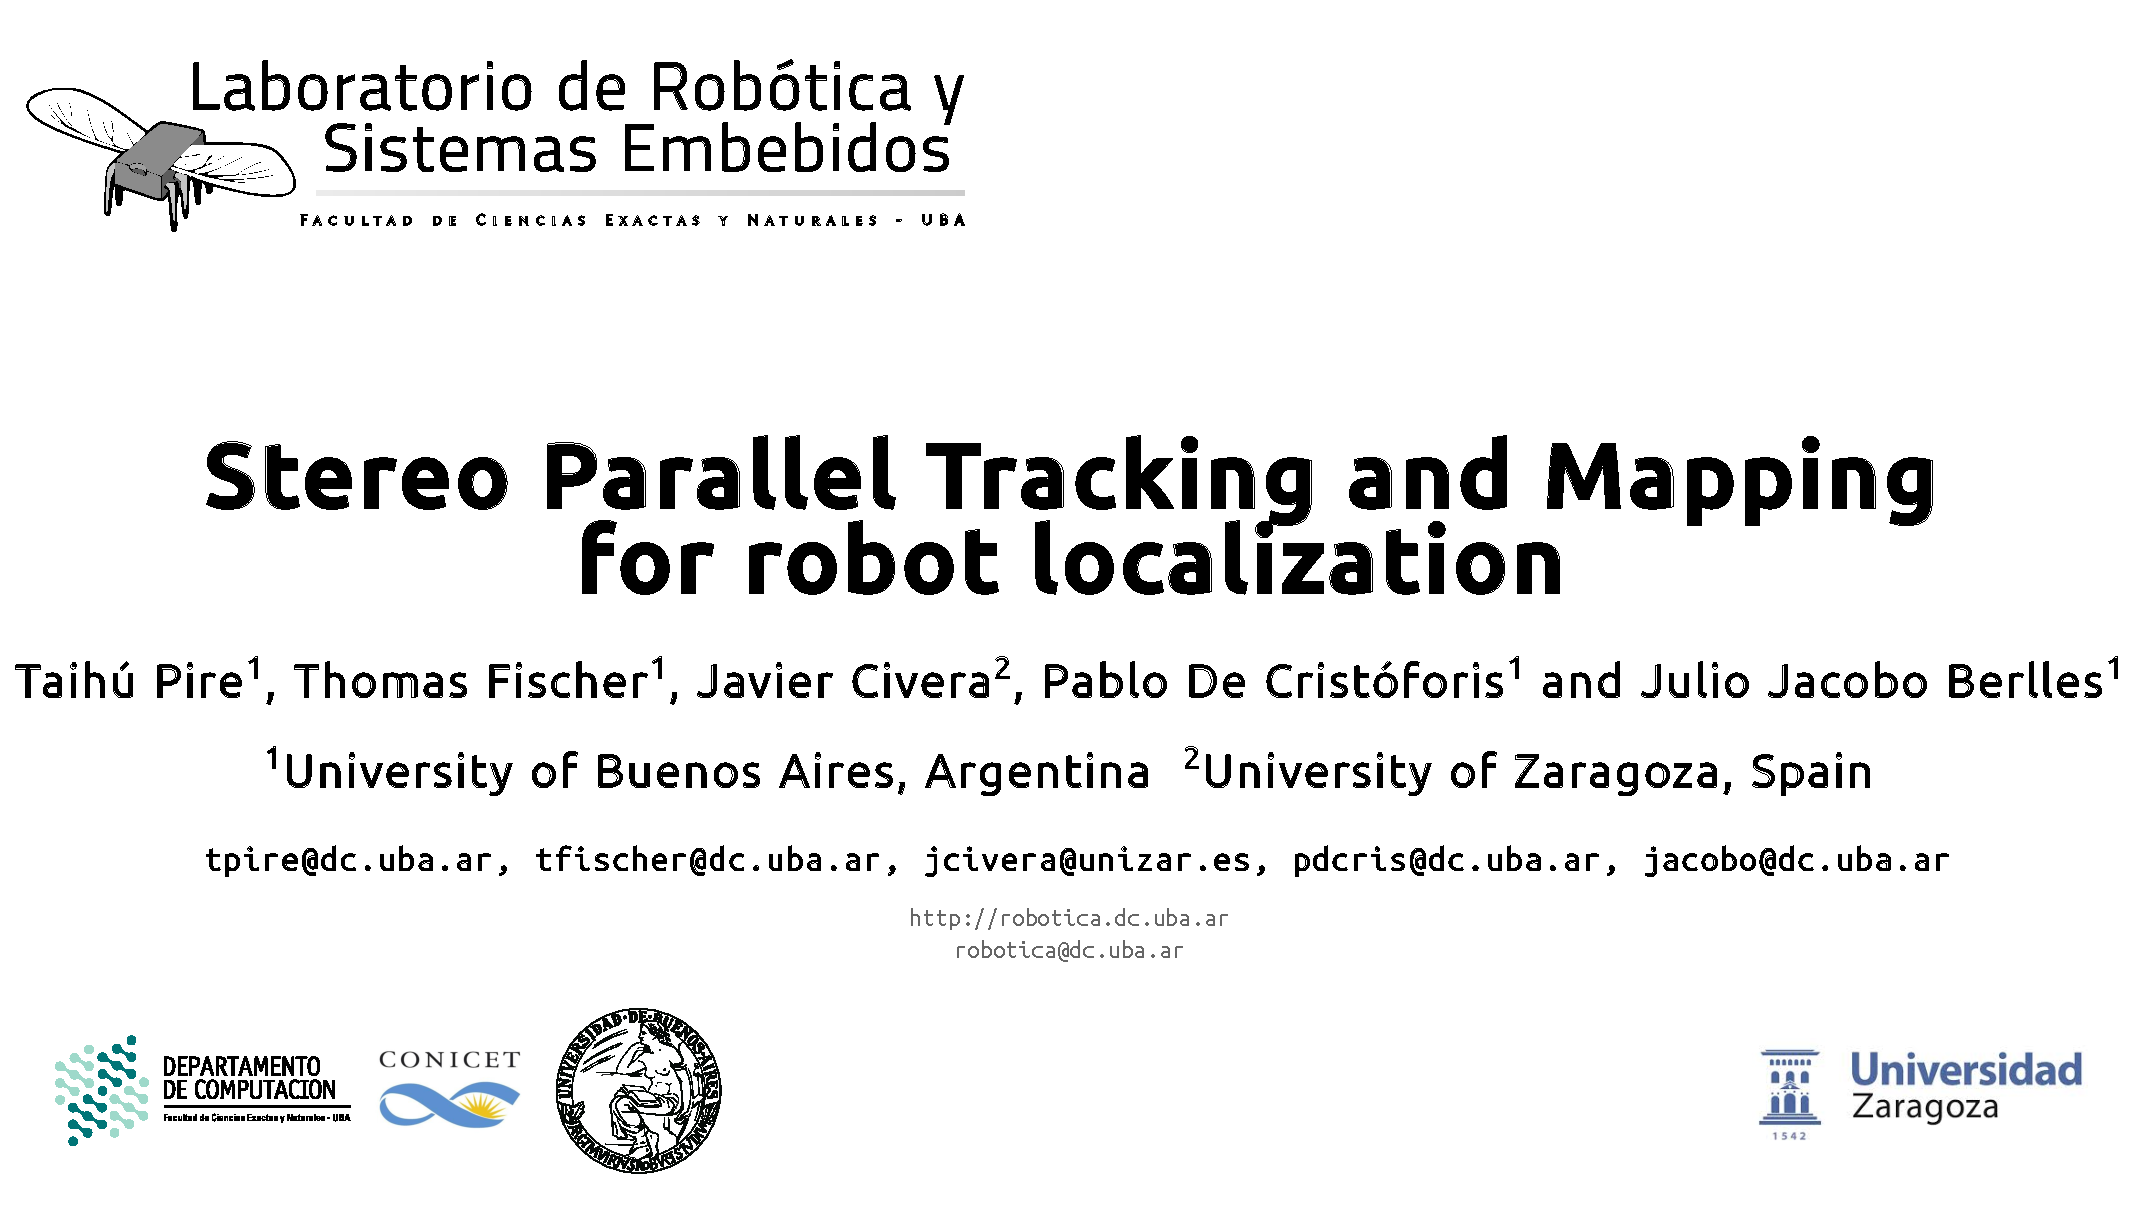
\includegraphics[width=1.0\columnwidth]{method/portada-sptam-kitti-video.pdf}
		\hfill
	\end{figure}

\end{frame}


% Frame ---------------------------------------------------------------------
\begin{frame}
    \frametitle{S-PTAM: Stereo Parallel Tracking and Mapping}
    Características:
    \begin{itemize}
    	\item Sensor: Cámara estéreo
		\item Construye y mantiene un mapa disperso del entorno.
		\item Basado en keyframes.
        \item Sistema SLAM basado en features.
        \item Fuertemente paralelizado: tracking, local mapping y loop closing.
        \item Real-time incluso en trayectorias largas.
        \item Código open-source en ROS (GPLv3) \url{https://github.com/lrse/sptam}
    \end{itemize}
\end{frame}


% Frame ---------------------------------------------------------------------
\begin{frame}
    \frametitle{S-PTAM en acción!}
    TODO: Agregar video de S-PTAM.
\end{frame}


\subsection{Funcionamiento}


% Frame ---------------------------------------------------------------------
\begin{frame}

	\frametitle{S-PTAM Denso}
	\begin{figure}[htb]
		\centering
		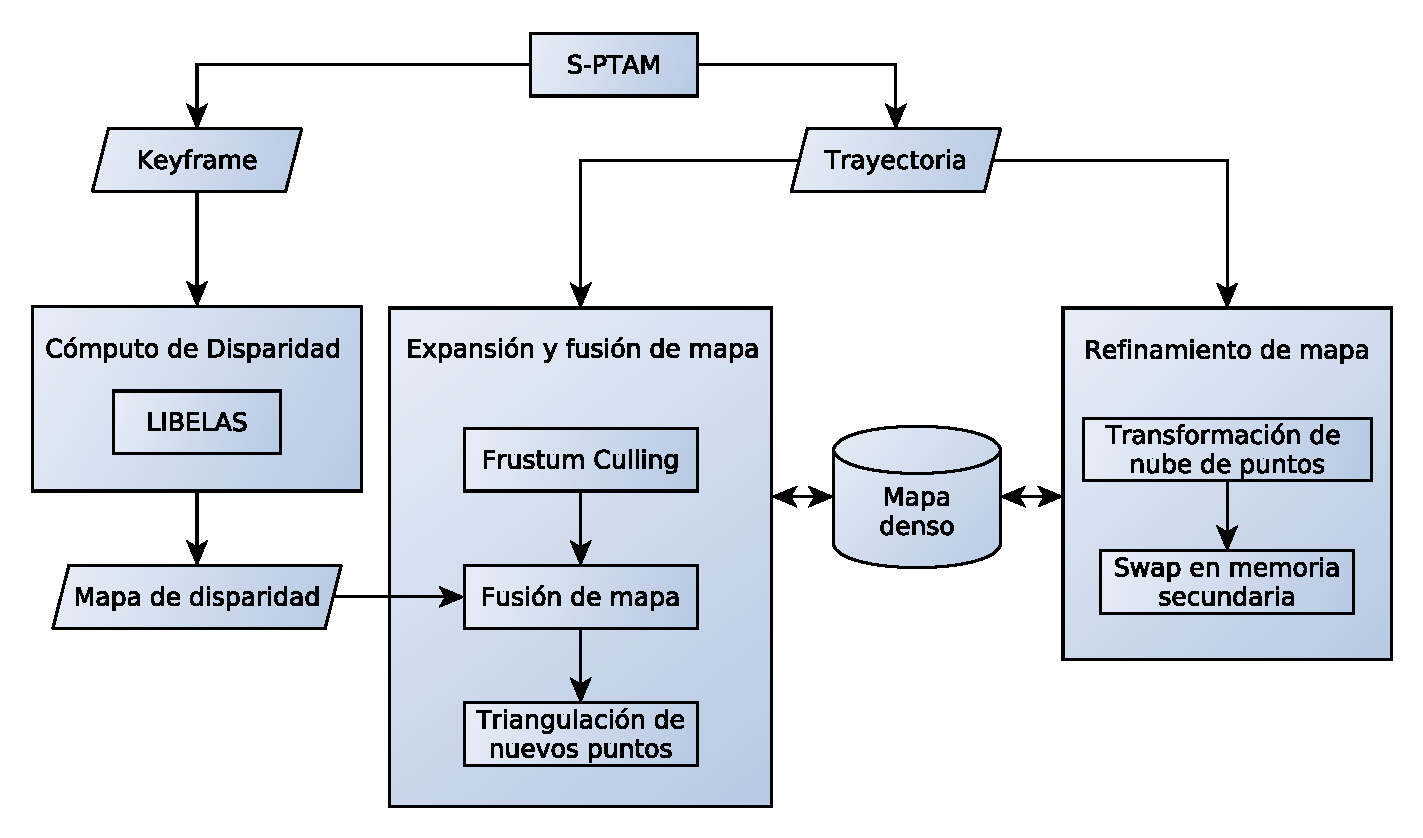
\includegraphics[width=1.0\columnwidth]{method/metodo-diagram.pdf}
		\hfill
	\end{figure}
\end{frame}


% Frame ---------------------------------------------------------------------
\begin{frame}
	\frametitle{Mapa de disparidad}

	\begin{itemize}
		\item Computa mapa de disparidad del \emph{keyframe} actual $\keyframe_{j}$.
	\end{itemize}
	
	\begin{figure}[htb]
		\centering
		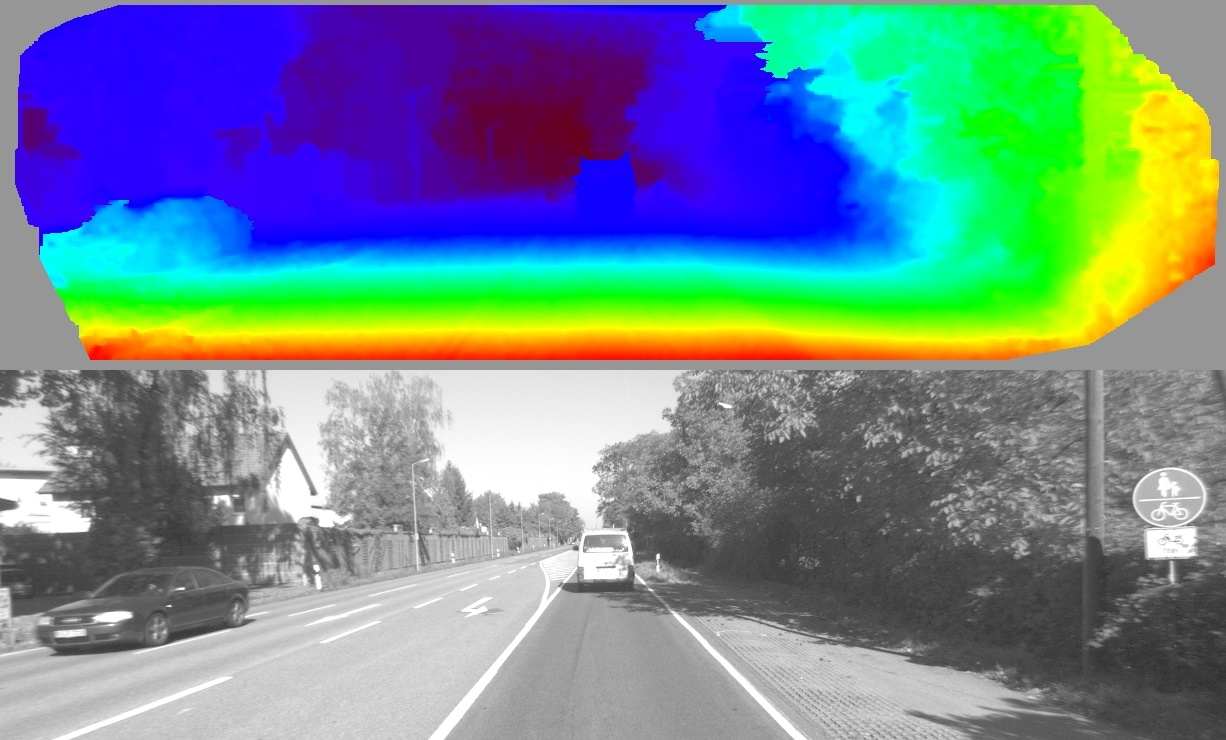
\includegraphics[width=0.4\columnwidth]{method/libelas_merge_kitti04_22.jpg}
		\caption{Mapa de disparidad LIBELAS - Dataset KITTI.}
	\end{figure}

	\begin{figure}[htb]
		\centering
		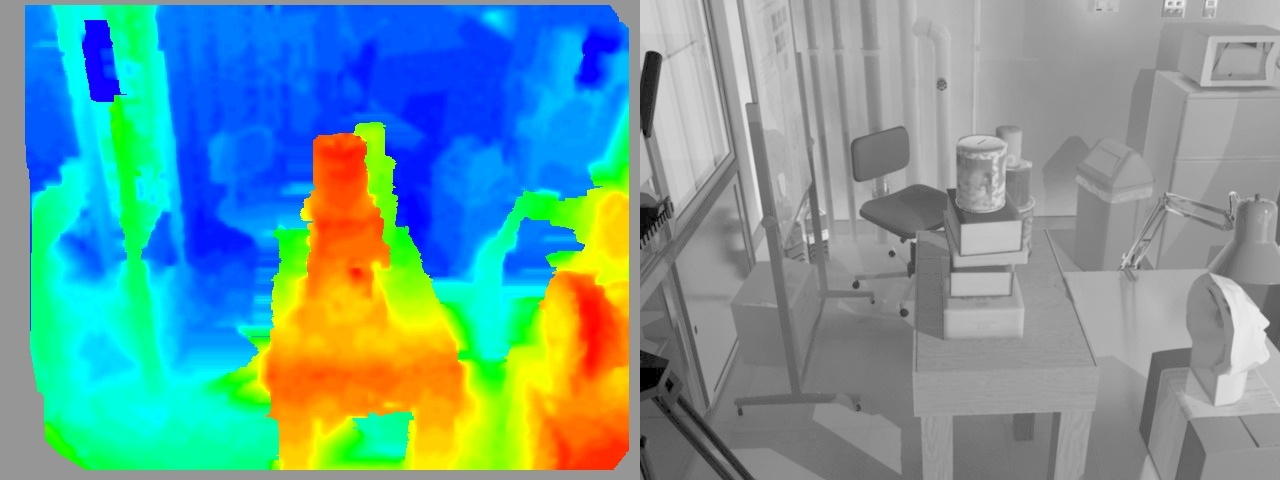
\includegraphics[width=0.4\columnwidth]{method/libelas_merge_tsukuba_222.jpg}
		\caption{Mapa de disparidad LIBELAS - Dataset Tsukuba.}
	\end{figure}

\end{frame}


% Frame ---------------------------------------------------------------------
\begin{frame}
	\frametitle{Expansión y fusión de mapa: Frustrum culling}
	
	\begin{itemize}
		\item Utilizando mapa de disparidad y posición del \emph{keyframe} actual $\keyframe_{j}$.
		\item \emph{Mapa local} a $\keyframe_{j}$: últimas $J$ \emph{nubes de puntos} $\left\{ \pointCloud_{j-J},\hdots,\pointCloud_{j}\right\}$.
		\item Aplicando \emph{Frustum culling} para filtrar puntos no-visibles desde $\keyframe_{j}$.
	\end{itemize}
	
	\begin{figure}[htb]
		\centering
		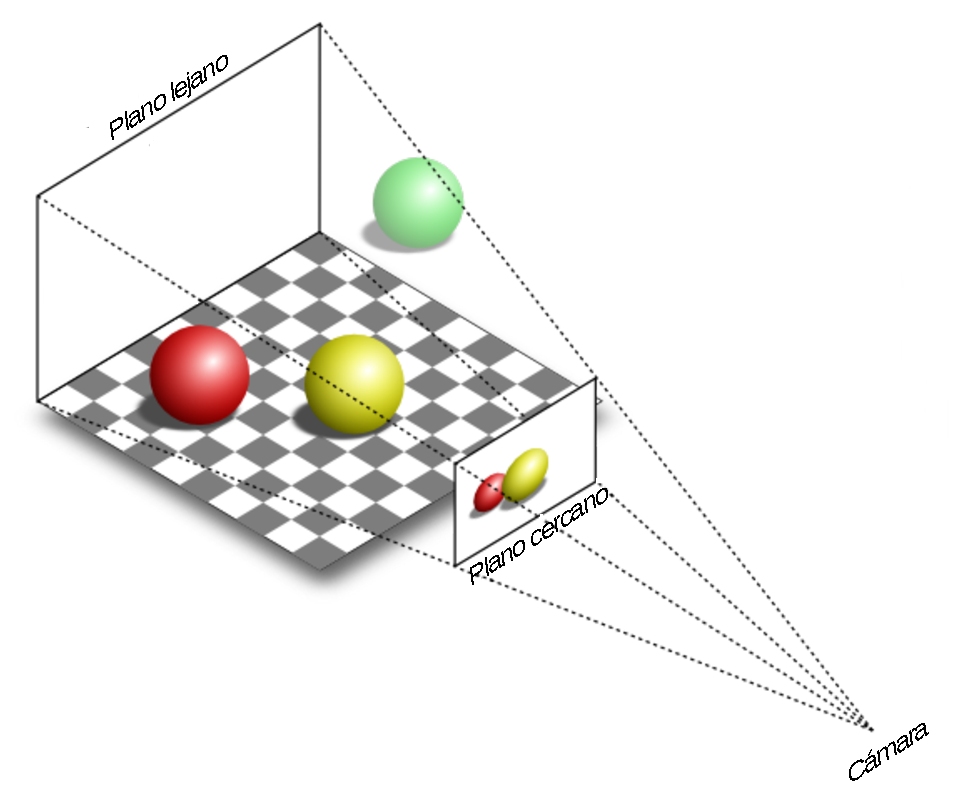
\includegraphics[width=0.6\columnwidth]{method/frustum_culling.pdf}
	\end{figure}

\end{frame}


% Frame ---------------------------------------------------------------------
\begin{frame}
	\frametitle{Expansión y fusión de mapa: Heurística de fusión}
	\begin{figure}[htb]
		\centering
		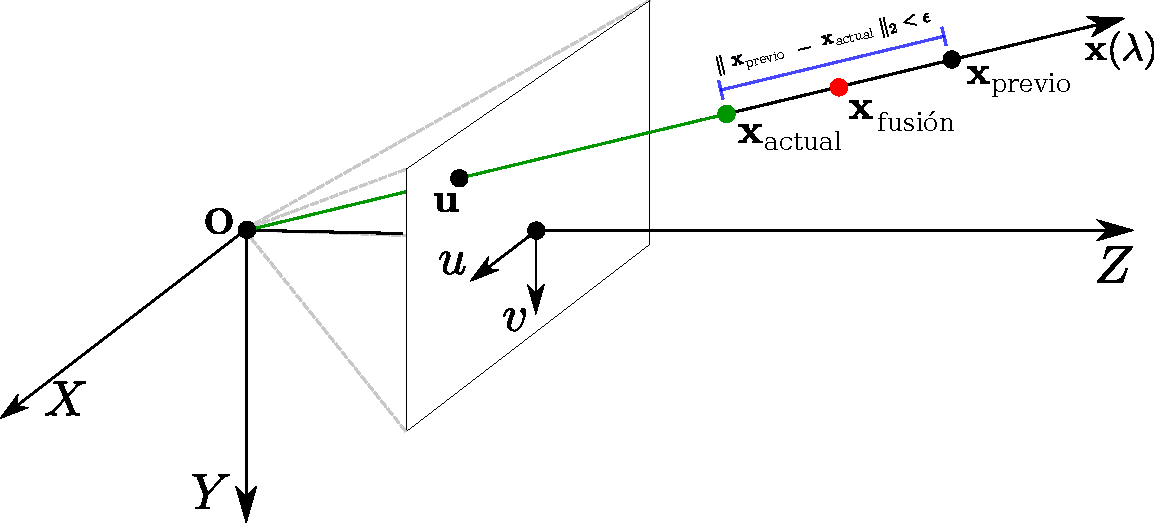
\includegraphics[width=\columnwidth]{method/metodo-fusion-spa.pdf}
	\end{figure}
	\begin{equation*}
		\point_{fusi\acute{o}n}=\frac{1}{\inverseDepth_{fusi\acute{o}n}}\frac{\point_{actual}}{\norm{\point_{actual}}}
		\quad \text{donde} \quad 
		\inverseDepth_{fusi\acute{o}n}=\frac{\inverseDepth_{actual}+\inverseDepth_{previo}}{2}
	\end{equation*}
\end{frame}


\section{Evaluación}


\subsection{Datasets}


% Frame ---------------------------------------------------------------------
\begin{frame}
	\frametitle{KITTI}
	\begin{figure}
		\subfloat[] {
			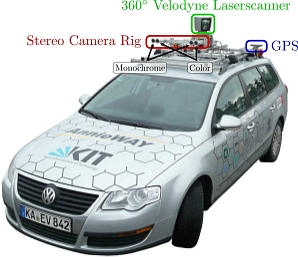
\includegraphics[width=0.3\columnwidth]{./images/kitti_sensors}
		}\hfill{}
		\subfloat[] {
			\begin{tabular}[b]{c}%
				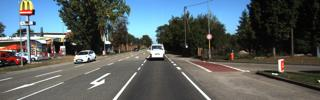
\includegraphics[width=0.3\columnwidth]{./images/kitti01}\thickspace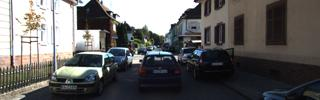
\includegraphics[width=0.3\columnwidth]{./images/kitti02}\\
				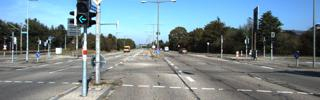
\includegraphics[width=0.3\columnwidth]{./images/kitti03}\thickspace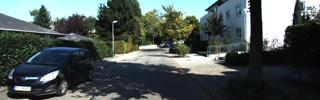
\includegraphics[width=0.3\columnwidth]{./images/kitti04}\\
				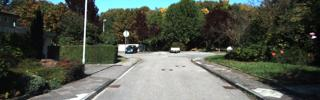
\includegraphics[width=0.3\columnwidth]{./images/kitti05}\thickspace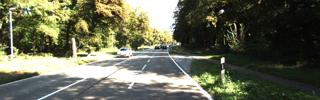
\includegraphics[width=0.3\columnwidth]{./images/kitti06}
			\end{tabular}
		}
	\end{figure}
\end{frame}


% Frame ---------------------------------------------------------------------
\begin{frame}
	\frametitle{Tsukuba}
	\begin{figure}
		\subfloat[] {
			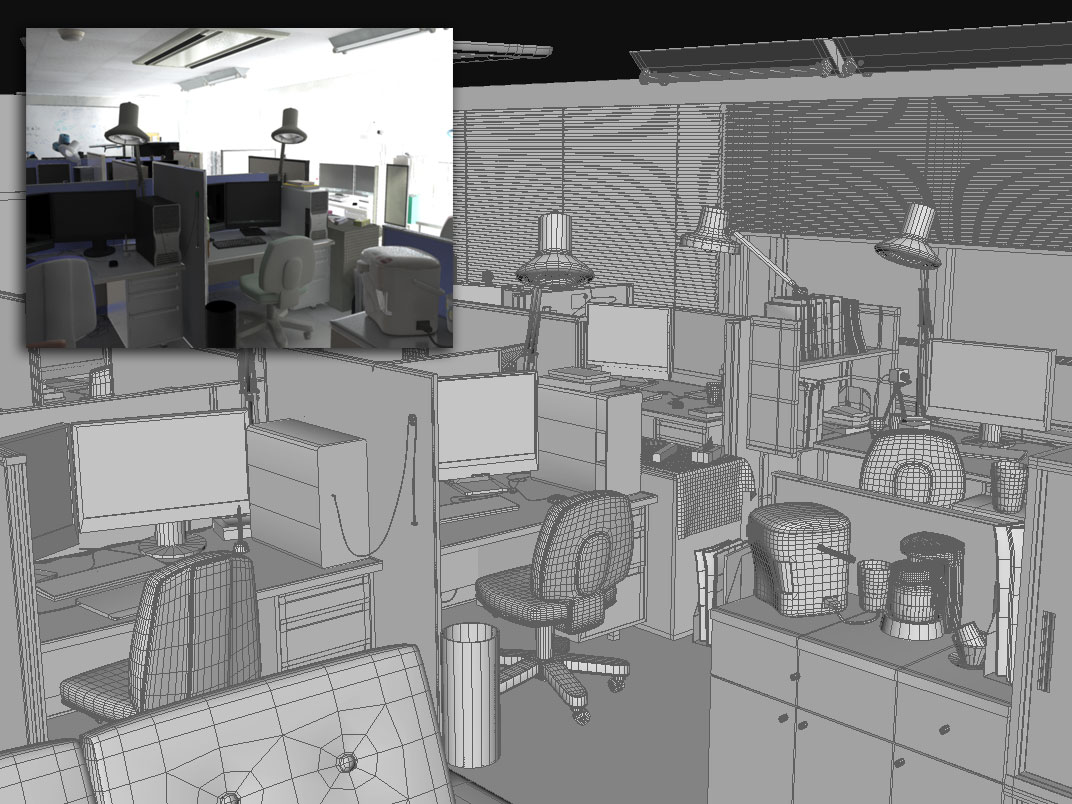
\includegraphics[width=0.4\columnwidth]{./images/tsukuba_dataset}
		}\hspace{0.2cm}
		\subfloat[] {
			\begin{tabular}[b]{c}%
				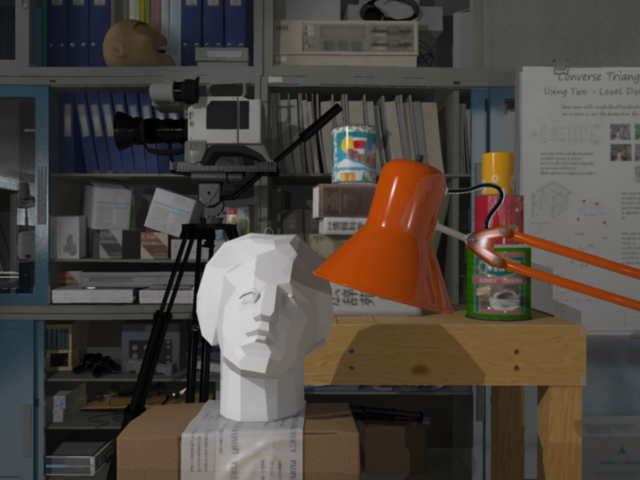
\includegraphics[width=0.2\columnwidth]{./images/tsukuba_sample1}\thickspace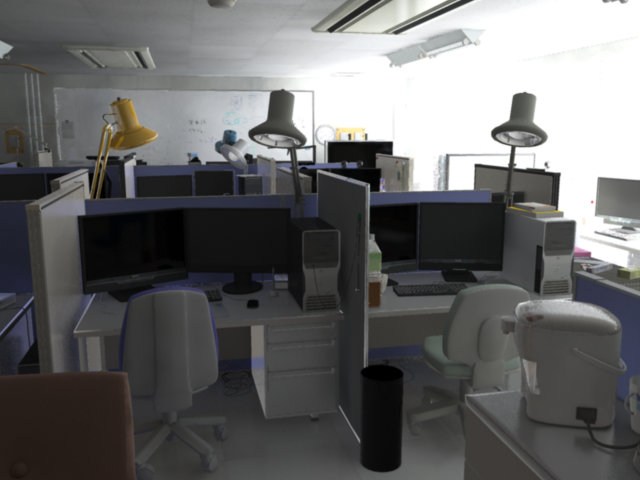
\includegraphics[width=0.2\columnwidth]{./images/tsukuba_sample2}\\
				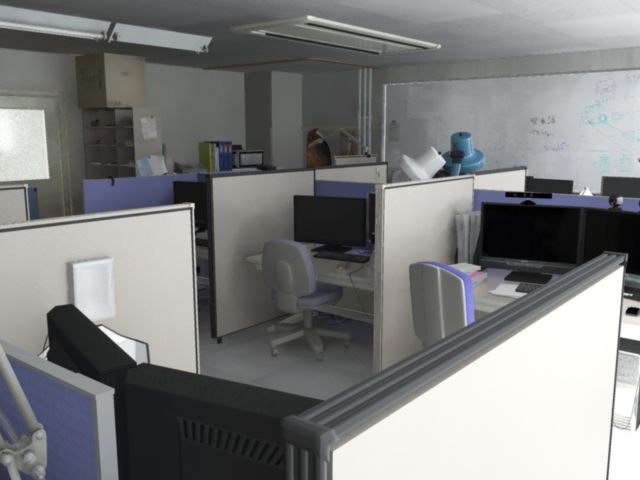
\includegraphics[width=0.2\columnwidth]{./images/tsukuba_sample3}\thickspace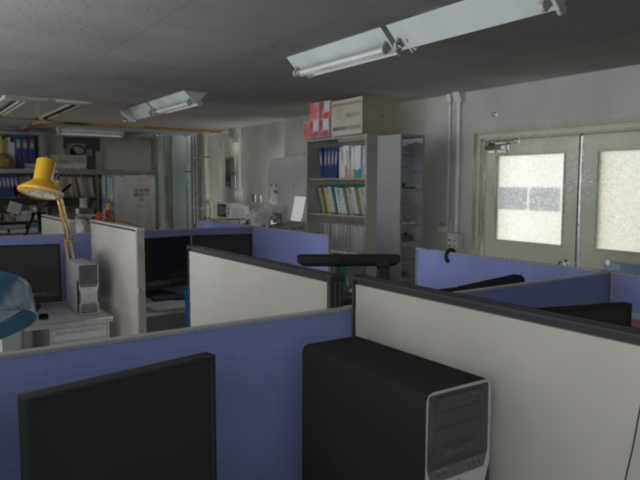
\includegraphics[width=0.2\columnwidth]{./images/tsukuba_sample4}
			\end{tabular}
		}
	\end{figure}
\end{frame}


% Frame ---------------------------------------------------------------------
\begin{frame}
	\frametitle{Ground truth - Mapas de profundidad}
\end{frame}


\subsection{Resultados}


% Frame ---------------------------------------------------------------------
\begin{frame}
	\frametitle{Reconstrucción 3D}
	\begin{figure}
		\subfloat[] {
			\begin{tabular}[b]{c}
				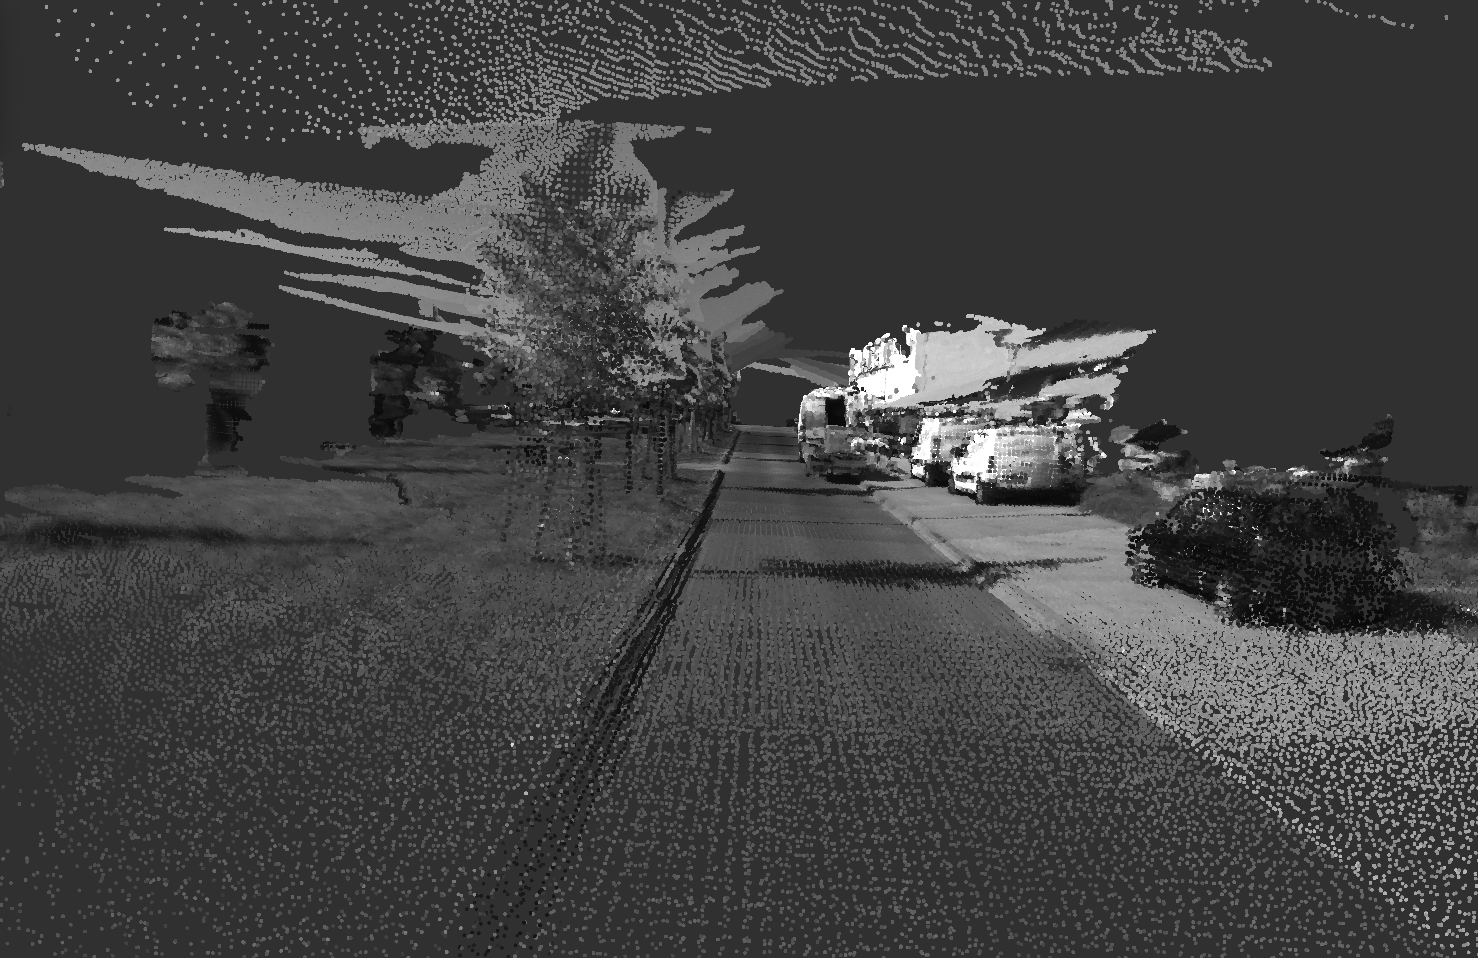
\includegraphics[width=0.3\columnwidth]{./images/kitti_3d_1}\thickspace
				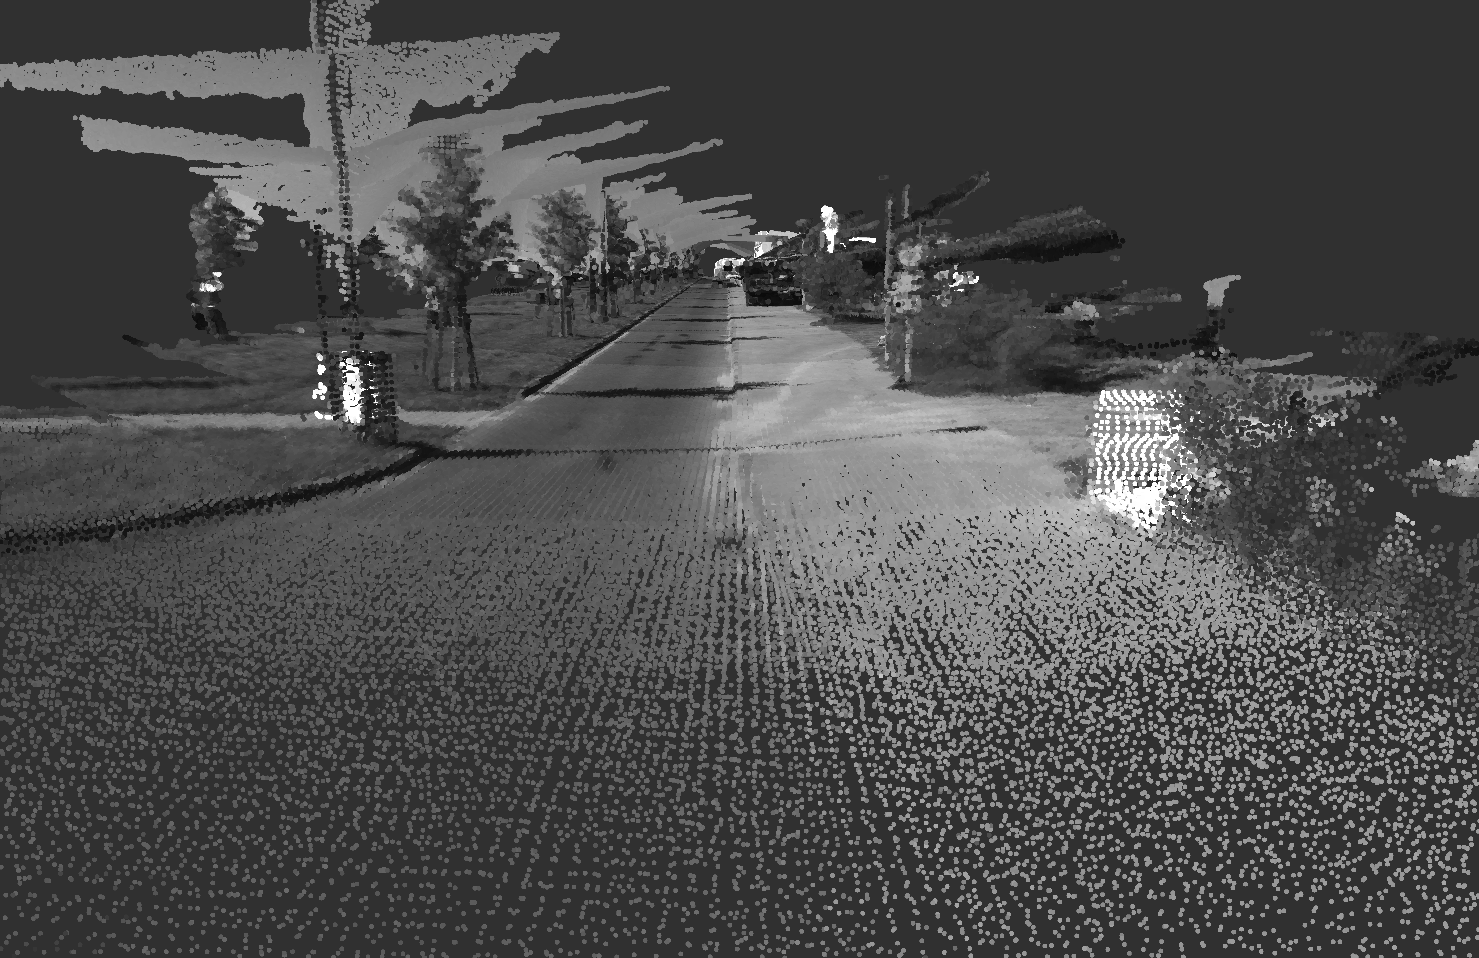
\includegraphics[width=0.3\columnwidth]{./images/kitti_3d_2}\thickspace
				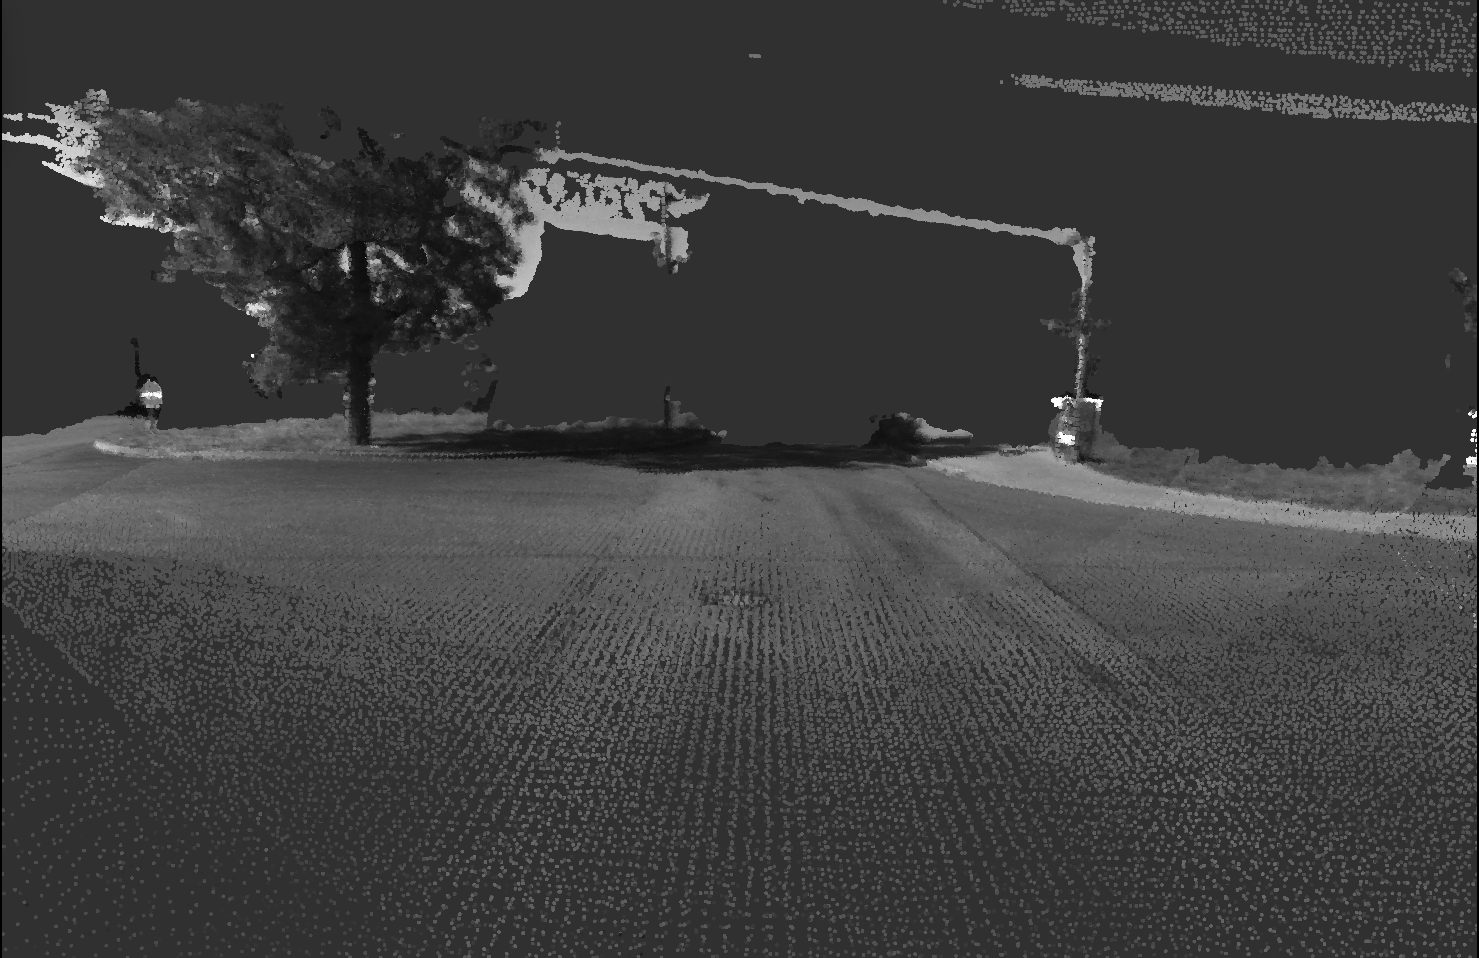
\includegraphics[width=0.3\columnwidth]{./images/kitti_3d_3}
			\end{tabular}
		}\vspace{0.1cm}
		\subfloat[] {
			\begin{tabular}[b]{c}
				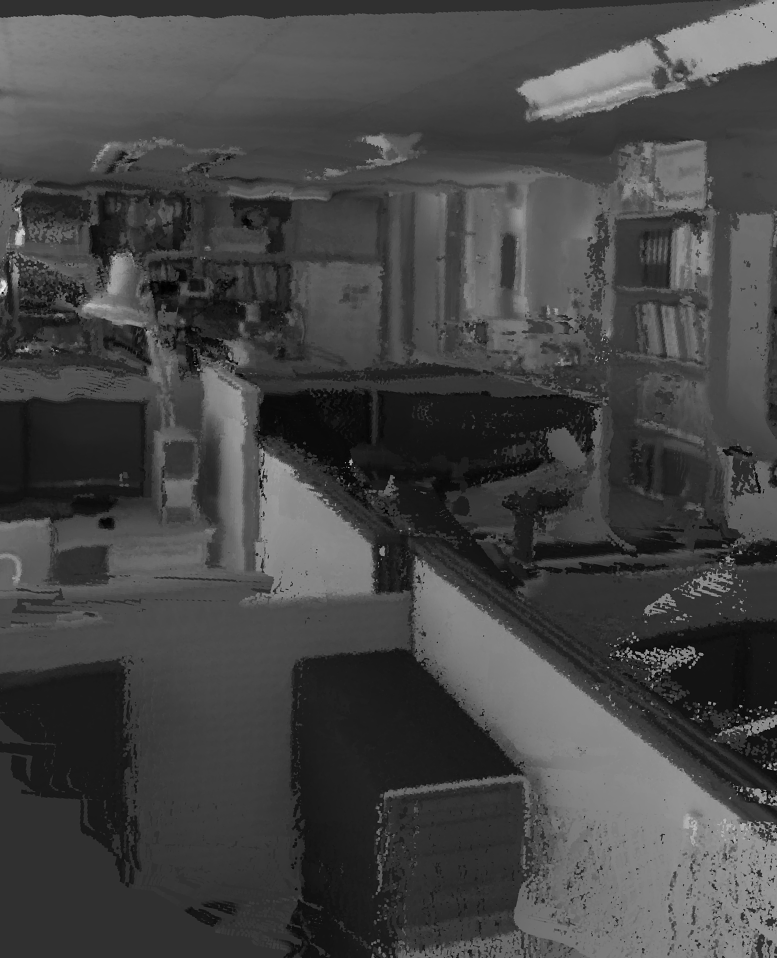
\includegraphics[width=0.3\columnwidth,height=3.0cm]{./images/tsukuba_3d_1}\thickspace
				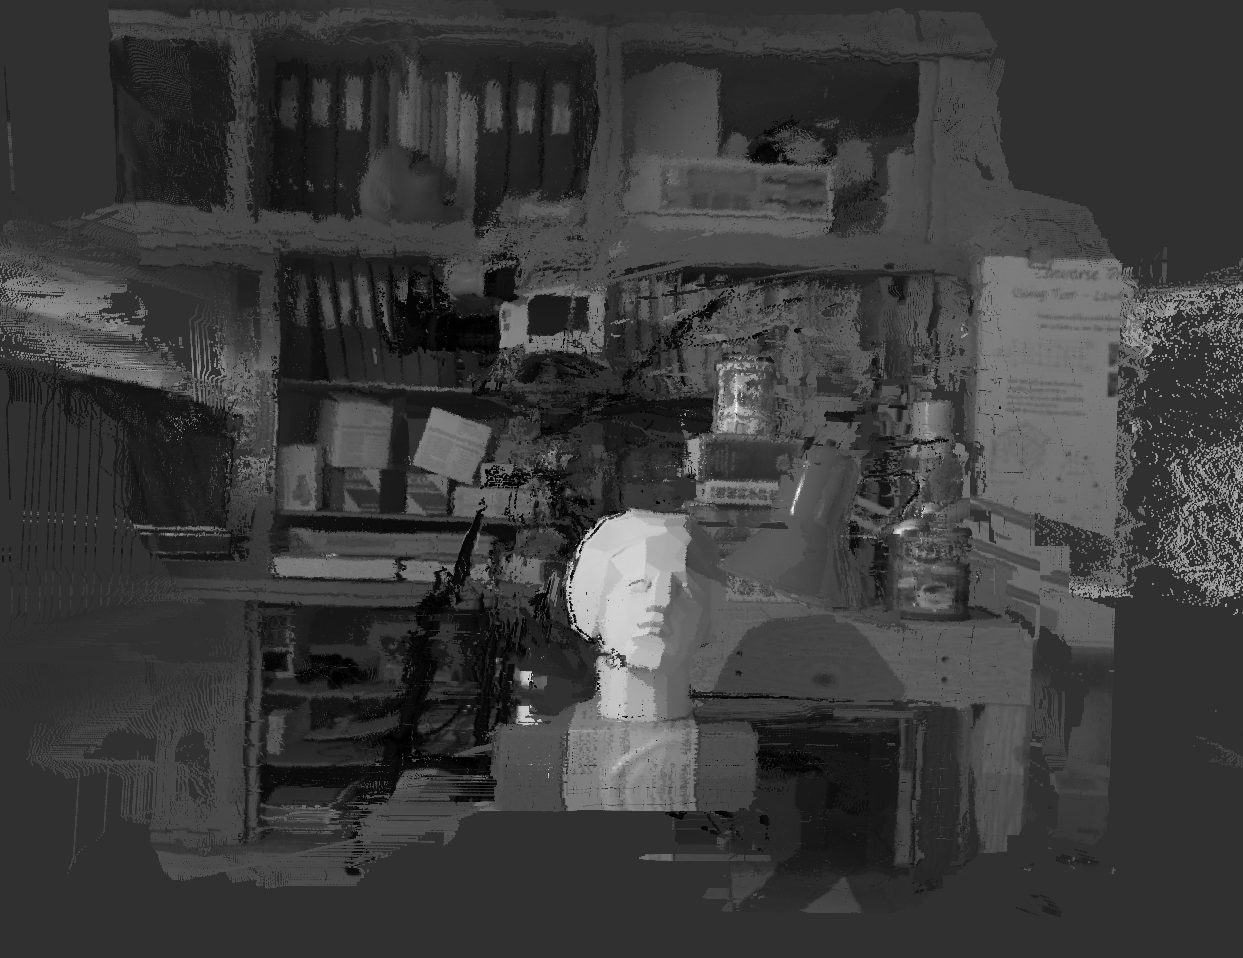
\includegraphics[width=0.3\columnwidth,height=3.0cm]{./images/tsukuba_3d_2}\thickspace
				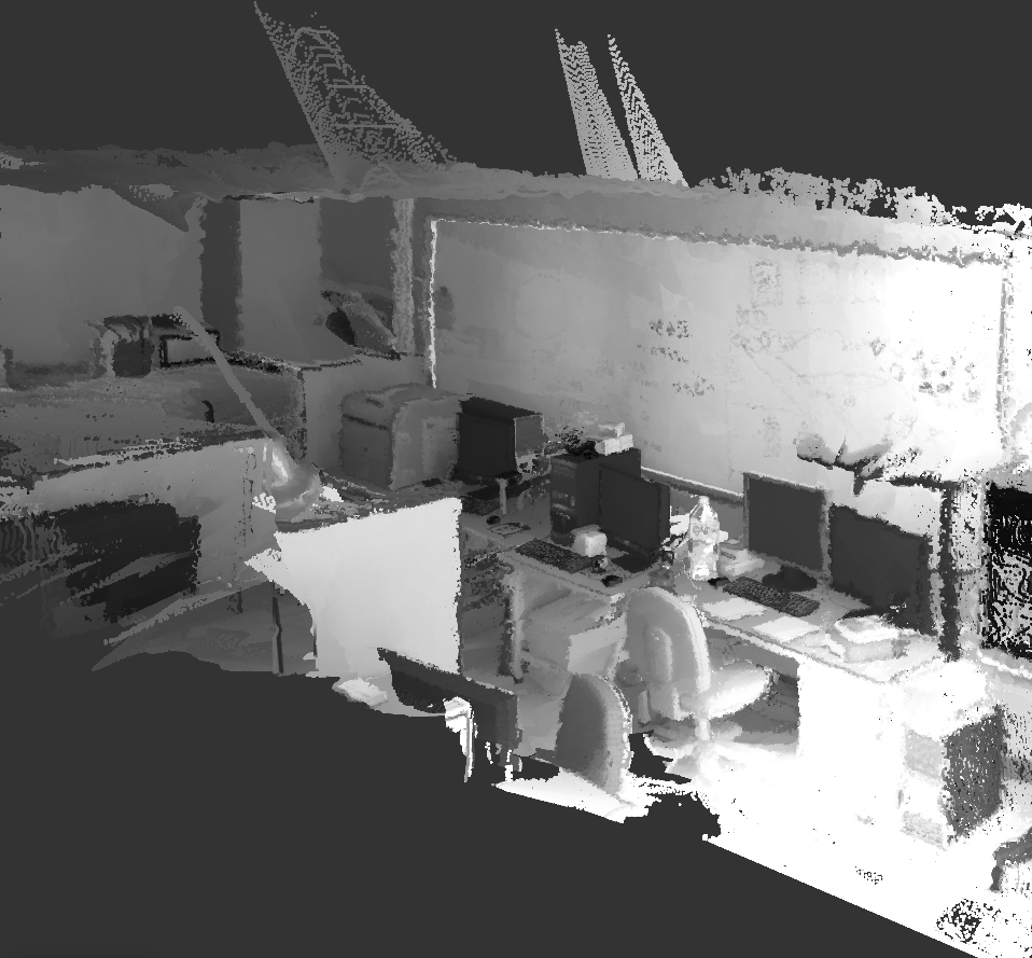
\includegraphics[width=0.3\columnwidth,height=3.0cm]{./images/tsukuba_3d_3}
			\end{tabular}
		}
	\end{figure}
\end{frame}


% Frame ---------------------------------------------------------------------
\begin{frame}
	\frametitle{KITTI: error de reconstrucción}
	\vspace{-2em}
	\begin{figure}
		\subfloat[Imagen izquierda]{
			\begin{tabular}[b]{c}
				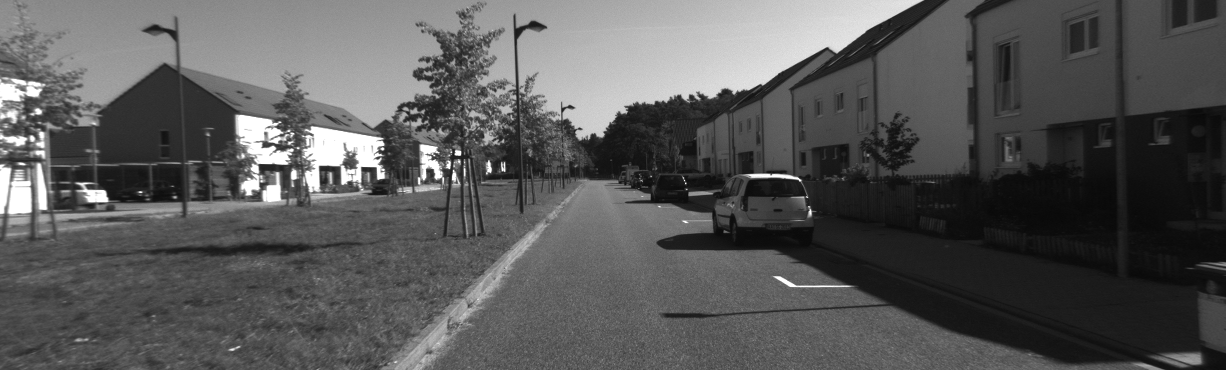
\includegraphics[width=0.45\columnwidth]{./experiments/kitti06_frame612_rgb.png}
			\end{tabular}
		}\thickspace
		\subfloat[Ground-Truth]{
			\begin{tabular}[b]{c}
				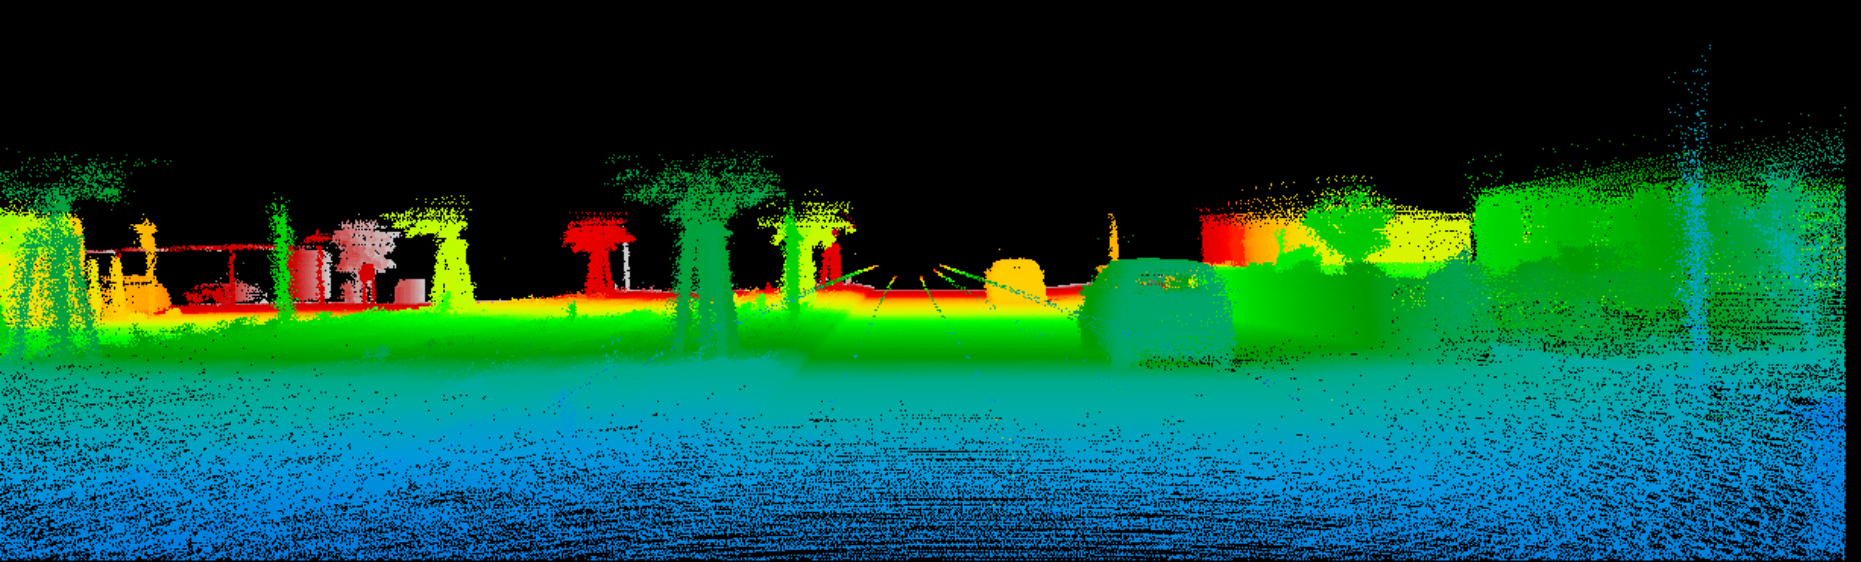
\includegraphics[width=0.45\columnwidth]{./experiments/kitti06_frame612_gt_high50.png}
			\end{tabular}
		}
	\end{figure}
	\vspace{-2em}
	\begin{figure}
		\subfloat[Mapa profundidad LIBELAS]{
			\begin{tabular}[b]{c}
				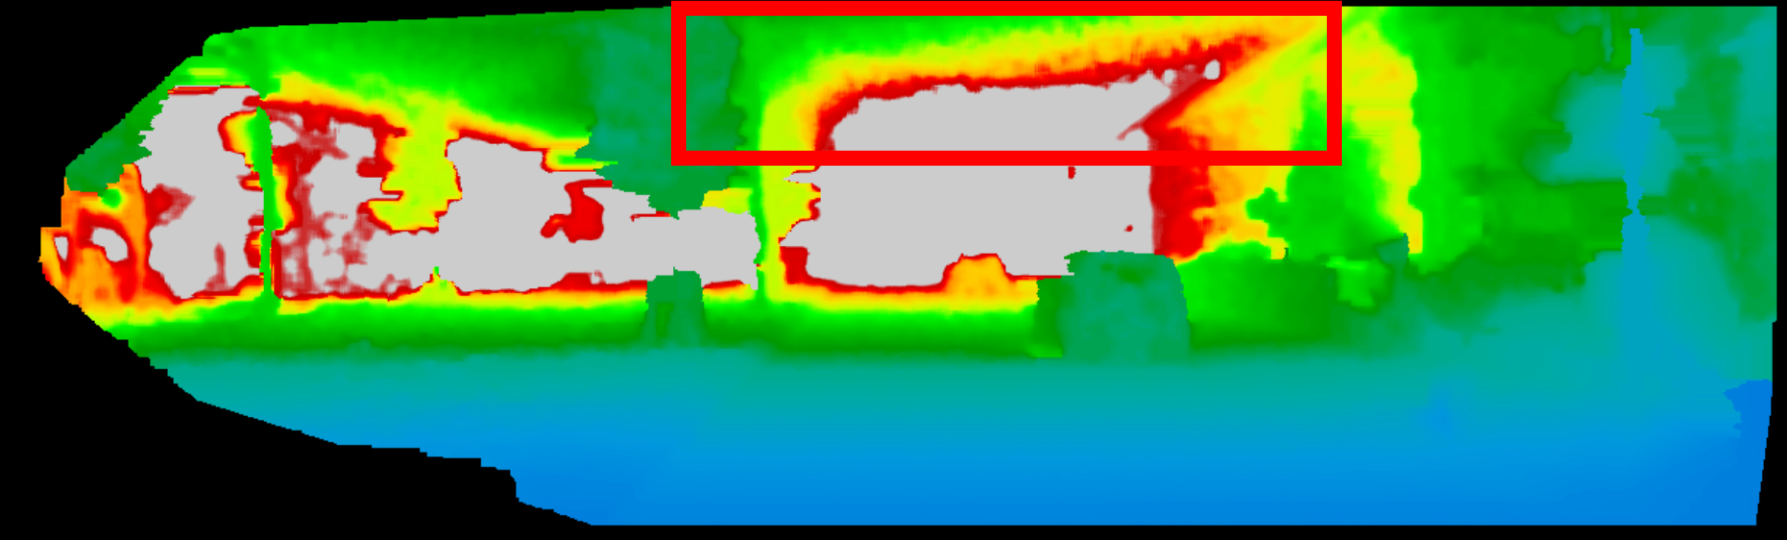
\includegraphics[width=0.45\columnwidth]{./experiments/kitti06_frame612_libelas_depth_high50-m.png}
			\end{tabular}
		}\thickspace
		\subfloat[Error mapa profundidad LIBELAS]{
			\begin{tabular}[b]{c}
				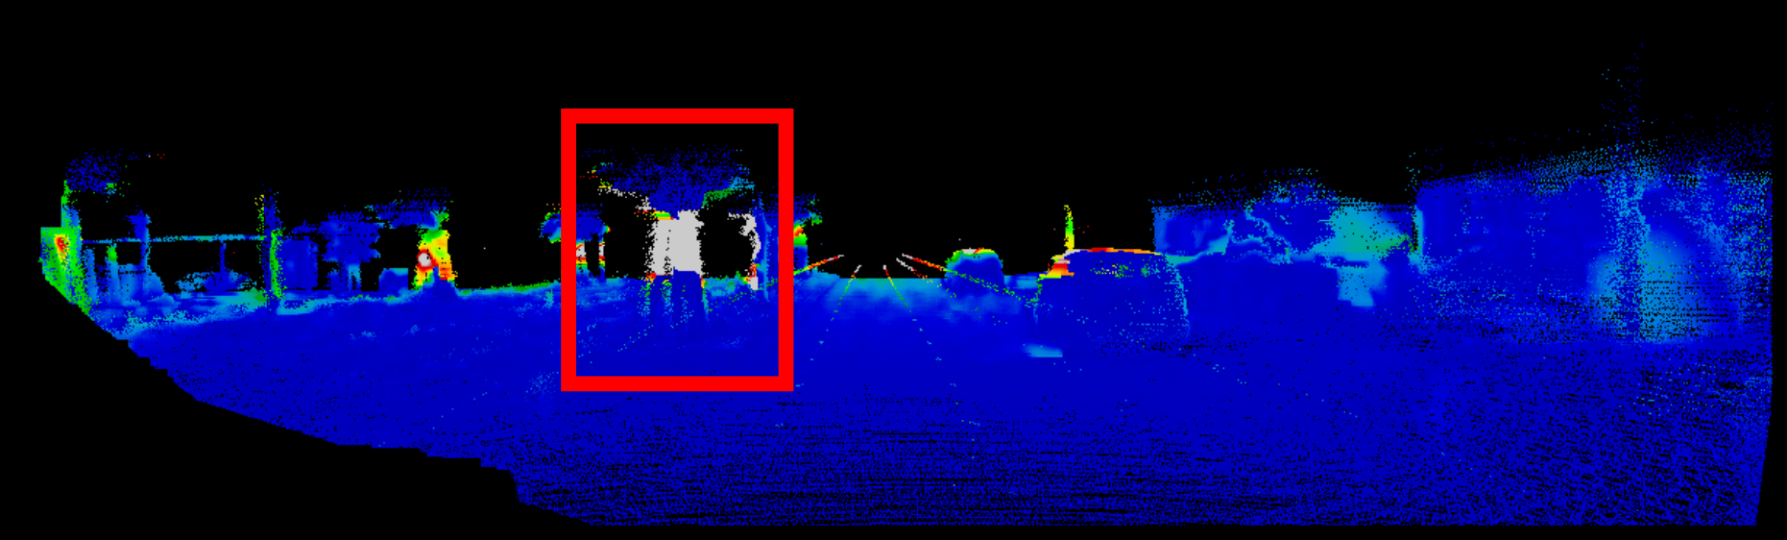
\includegraphics[width=0.45\columnwidth]{./experiments/kitti06_frame612_libelas_error_high50-m.png}
			\end{tabular}
		}
	\end{figure}
	\vspace{-2em}
	\begin{figure}
		\subfloat[Mapa profundidad S-PTAM Denso]{
			\begin{tabular}[b]{c}
				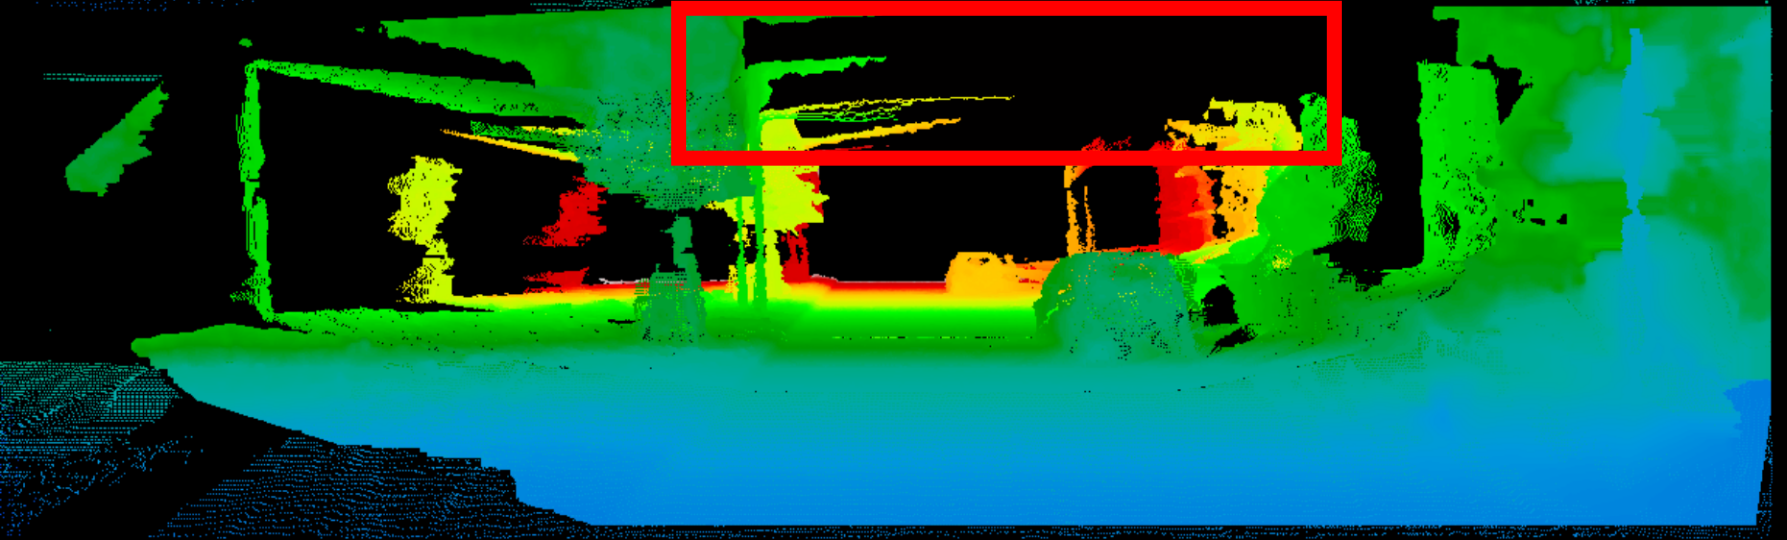
\includegraphics[width=0.45\columnwidth]{./experiments/kitti06_frame612_dense_high50-m.png}
			\end{tabular}
		}\thickspace
		\subfloat[Error mapa profundidad S-PTAM Denso]{
			\begin{tabular}[b]{c}
				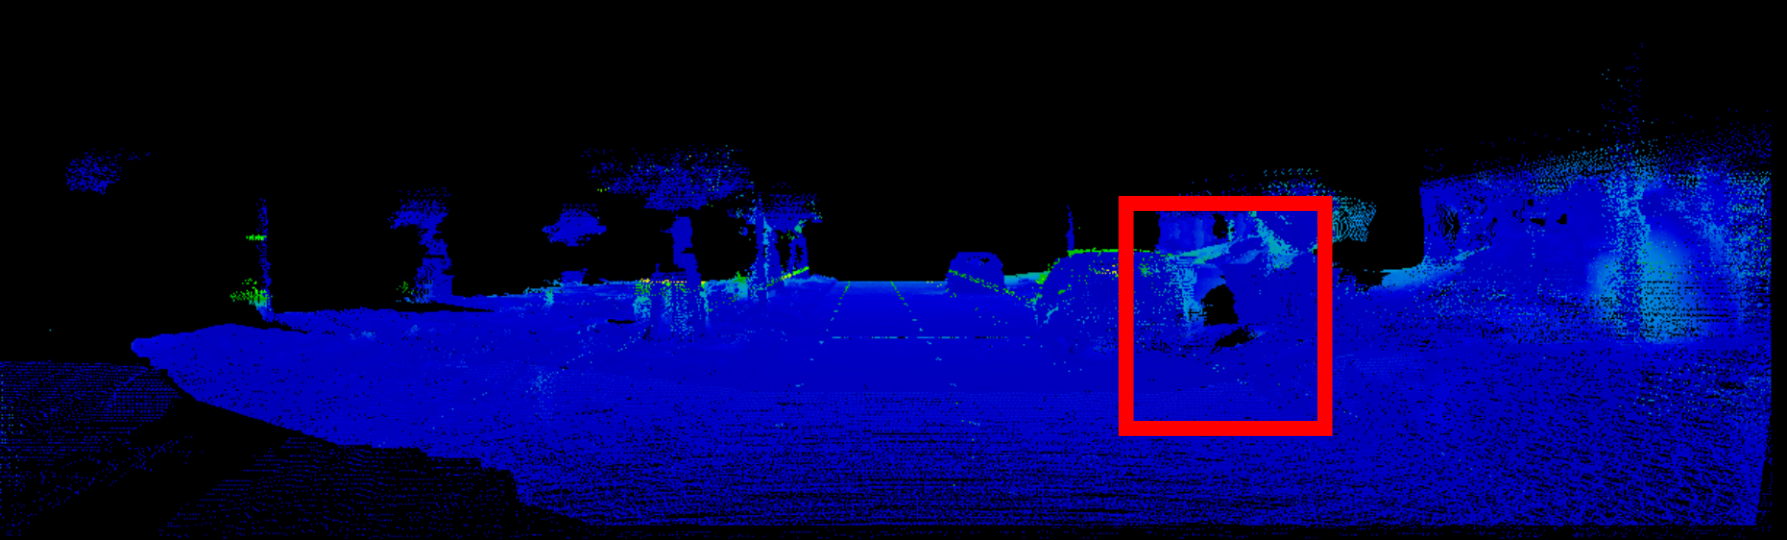
\includegraphics[width=0.45\columnwidth]{./experiments/kitti06_frame612_error_high50-m.png}
			\end{tabular}
		}
	\end{figure}
	\vspace{-2em}
	\begin{figure}
		\subfloat[]{
			\begin{tabular}[b]{c}
				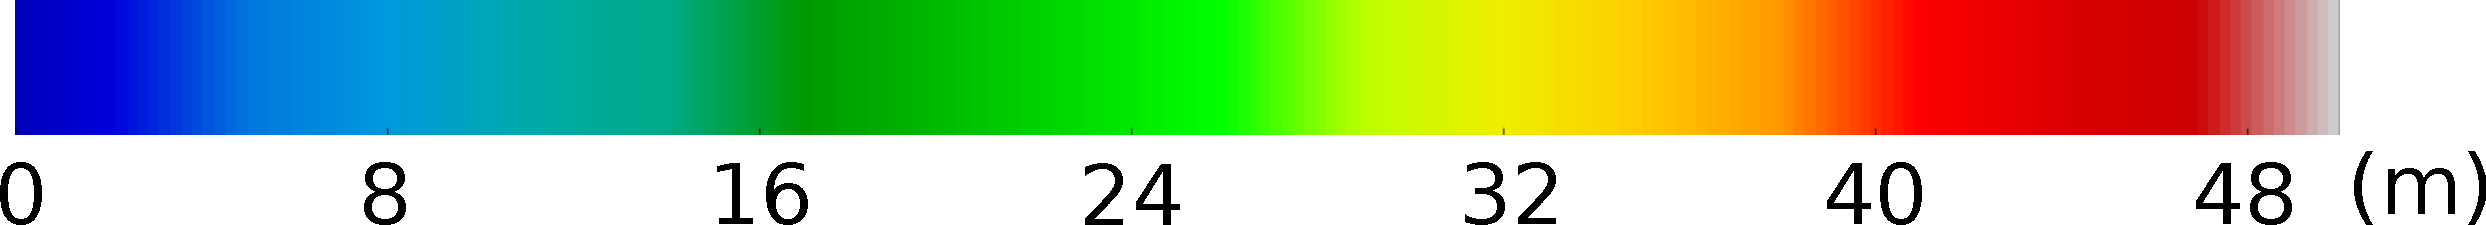
\includegraphics[width=0.60\columnwidth]{./experiments/high50_bar.pdf}
			\end{tabular}
		}
	\end{figure}
\end{frame}


% Frame ---------------------------------------------------------------------
\begin{frame}
	\frametitle{Tsukuba: error de reconstrucción}
	\vspace{-1em}
	\begin{figure}
		\captionsetup{justification=centering}
		\subfloat[Imagen izquierda]{
			\begin{tabular}[b]{c}
				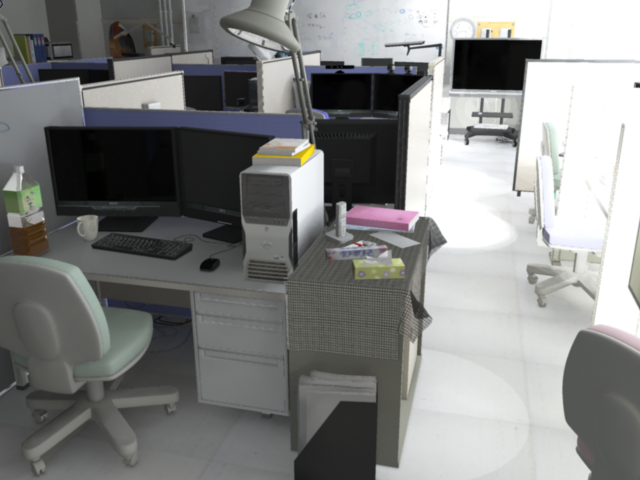
\includegraphics[width=0.25\columnwidth]{./experiments/tsukuba_frame807_rgb.png}
			\end{tabular}
		}\thickspace
		\subfloat[Mapa profundidad LIBELAS]{
			\begin{tabular}[b]{c}
				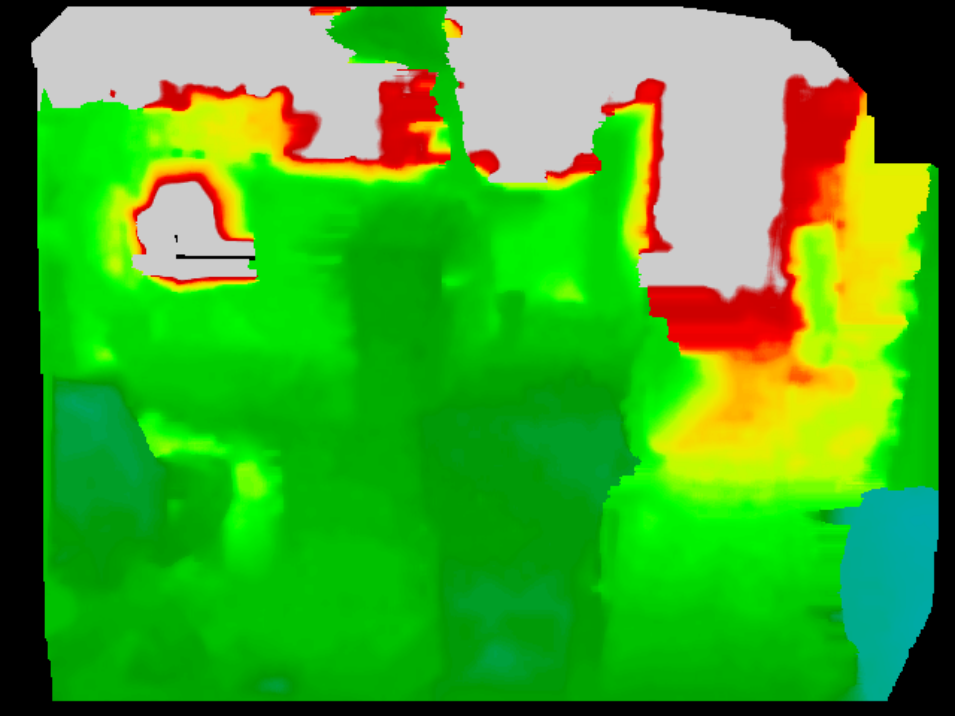
\includegraphics[width=0.25\columnwidth]{./experiments/tsukuba_frame807_libelas_depth_high6.png}
			\end{tabular}
		}\thickspace
		\subfloat[Mapa profundidad S-PTAM Denso]{
			\begin{tabular}[b]{c}
				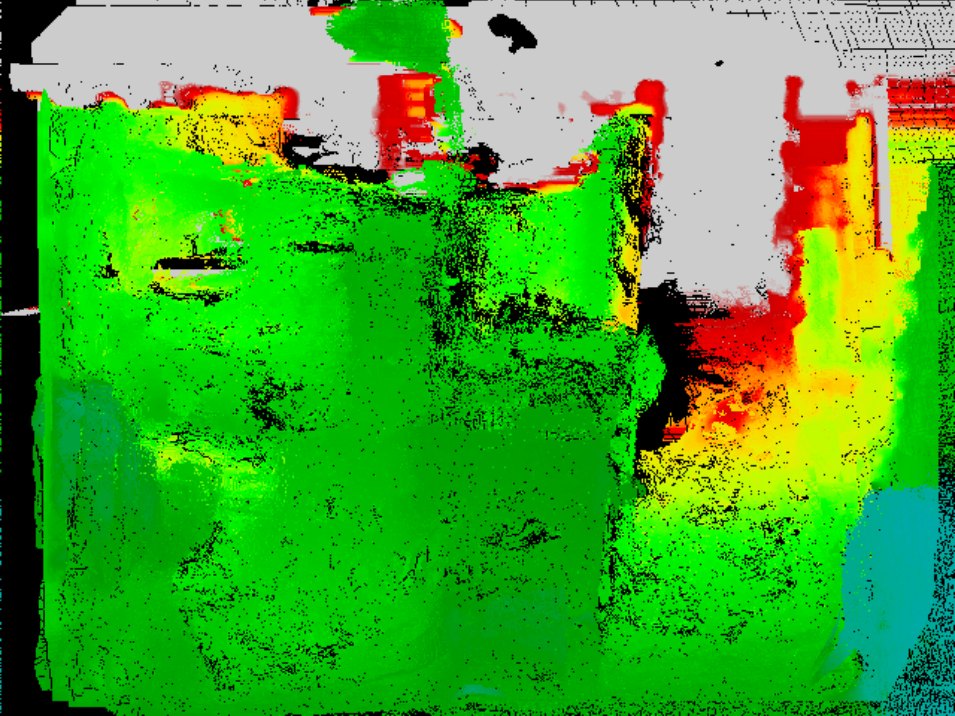
\includegraphics[width=0.25\columnwidth]{./experiments/tsukuba_frame807_dense_high6.png}
			\end{tabular}
		}
	\end{figure}
	\vspace{-2em}
	\begin{figure}
		\captionsetup{justification=centering}
		\subfloat[Ground-Truth]{
			\begin{tabular}[b]{c}
				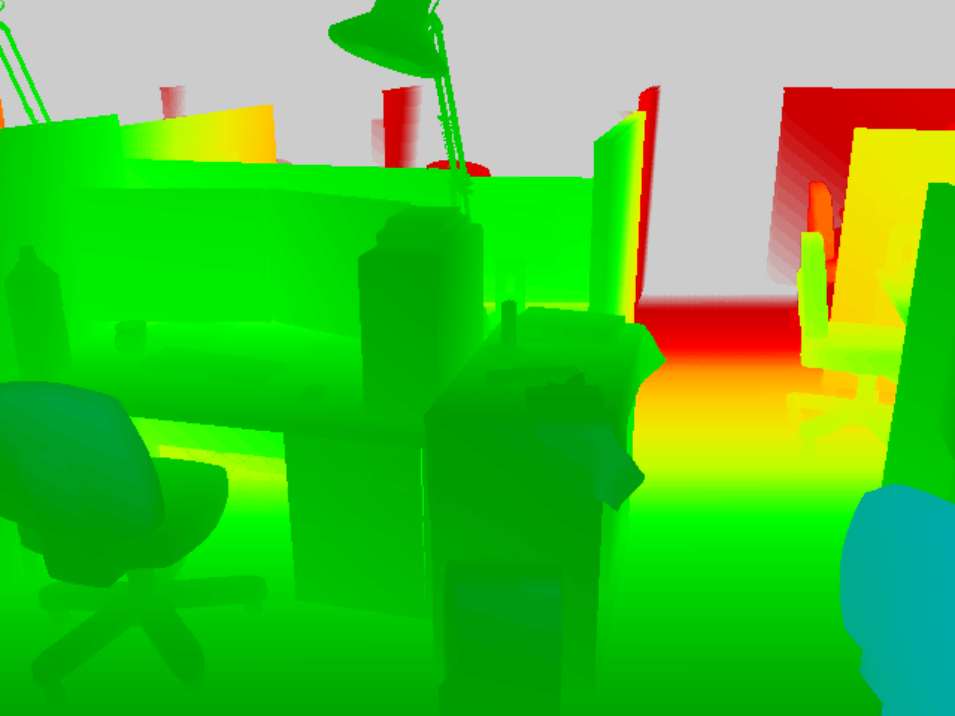
\includegraphics[width=0.25\columnwidth]{experiments/tsukuba_frame807_gt_high6.png}
			\end{tabular}
		}\thickspace
		\subfloat[Error mapa profundidad LIBELAS]{
			\begin{tabular}[b]{c}
				\includegraphics[width=0.25\columnwidth]{./experiments/tsukuba_frame807_libelas_error_high6-m.png}
			\end{tabular}
		}\thickspace
		\subfloat[Error mapa profundidad S-PTAM Denso]{
			\begin{tabular}[b]{c}
				\includegraphics[width=0.25\columnwidth]{./experiments/tsukuba_frame807_error_high6-m.png}
			\end{tabular}
		}
	\end{figure}
	\vspace{-2em}
	\begin{figure}
		\subfloat[]{
			\begin{tabular}[b]{c}
				\includegraphics[width=0.60\columnwidth]{./experiments/high6_bar.pdf}
			\end{tabular}
		}
	\end{figure}
\end{frame}


% Frame ---------------------------------------------------------------------
\begin{frame}
	\frametitle{KITTI 06: error de mediana}
	\centering
	Error (profundidad vs. error) en la secuencia 06 del Dataset KITTI.
	\begin{figure}[!htb]
		\captionsetup{justification=centering}
		\subfloat[Error en LIBELAS]{\includegraphics[width=0.48\columnwidth]{./experiments/kitti06_libelas_boxplot.png}%
		}
		\hfil
		\subfloat[Error en S-PTAM Denso]{\includegraphics[width=0.48\columnwidth]{./experiments/kitti06_dense_boxplot.png}%
		}
	\end{figure}
\end{frame}


% Frame ---------------------------------------------------------------------
\begin{frame}
	\frametitle{KITTI 06: error de mediana}
	\vspace{-2em}
	\begin{figure}[!htb]
		\captionsetup{justification=centering}
		\subfloat[Comparación de mediana de error entre LIBELAS y S-PTAM Denso (profundidad vs. error) en la secuencia 06 del Dataset KITTI.] {
			\includegraphics[width=0.8\columnwidth]{./experiments/medians_comparison_kitti.png}%
		}
	\end{figure}
\end{frame}


% Frame ---------------------------------------------------------------------
\begin{frame}
	\frametitle{Tsukuba: error de mediana}
	\centering
	Error (profundidad vs. error) en el Dataset Tsukuba.
	\begin{figure}[!htb]
		\captionsetup{justification=centering}
		\subfloat[Error en LIBELAS]{\includegraphics[width=0.48\columnwidth]{./experiments/tsukuba_libelas_boxplot.png}%
		}
		\hfil
		\subfloat[Error en S-PTAM Denso]{\includegraphics[width=0.48\columnwidth]{./experiments/tsukuba_dense_boxplot.png}%
		}
	\end{figure}
\end{frame}


% Frame ---------------------------------------------------------------------
\begin{frame}
	\frametitle{Tsukuba: error de mediana}
	\vspace{-2em}
	\begin{figure}[!htb]
		\captionsetup{justification=centering}
		\subfloat[Comparación de mediana de error entre LIBELAS y S-PTAM Denso (profundidad vs. error) en el Dataset Tsukuba.] {
			\includegraphics[width=0.8\columnwidth]{./experiments/medians_comparison_tsukuba.png}%
		}
	\end{figure}
\end{frame}


% Frame ---------------------------------------------------------------------
\begin{frame}
	\frametitle{KITTI: error de mediana}
	\centering
	Comparación de mediana de error (profundidad vs. error).
	\vspace{-1em}
	\begin{figure}[!htb]
		\captionsetup{justification=centering}
		\subfloat[KITTI 00]{\includegraphics[width=0.35\columnwidth]{./experiments/kitti_medians/00.png}%
		}
		\hfil
		\subfloat[KITTI 01]{\includegraphics[width=0.35\columnwidth]{./experiments/kitti_medians/01.png}%
		}
	\end{figure}
	\vspace{-2em}
	\begin{figure}[!htb]
		\captionsetup{justification=centering}
		\subfloat[KITTI 02]{\includegraphics[width=0.35\columnwidth]{./experiments/kitti_medians/02.png}%
		}
		\hfil
		\subfloat[KITTI 03]{\includegraphics[width=0.35\columnwidth]{./experiments/kitti_medians/03.png}%
		}
	\end{figure}
\end{frame}


% Frame ---------------------------------------------------------------------
\begin{frame}
	\frametitle{KITTI: error de mediana}
	\centering
	Comparación de mediana de error (profundidad vs. error).
	\vspace{-1em}
	\begin{figure}[!htb]
		\captionsetup{justification=centering}
		\subfloat[KITTI 04]{\includegraphics[width=0.35\columnwidth]{./experiments/kitti_medians/04.png}%
		}
		\hfil
		\subfloat[KITTI 05]{\includegraphics[width=0.35\columnwidth]{./experiments/kitti_medians/05.png}%
		}
	\end{figure}
	\vspace{-2em}
	\begin{figure}[!htb]
		\captionsetup{justification=centering}
		\subfloat[KITTI 07]{\includegraphics[width=0.35\columnwidth]{./experiments/kitti_medians/07.png}%
		}
		\hfil
		\subfloat[KITTI 08]{\includegraphics[width=0.35\columnwidth]{./experiments/kitti_medians/08.png}%
		}
	\end{figure}
\end{frame}


% Frame ---------------------------------------------------------------------
\begin{frame}
	\frametitle{KITTI: error de mediana}
	\centering
	Comparación de mediana de error (profundidad vs. error).
	\vspace{-1em}
	\begin{figure}[!htb]
		\captionsetup{justification=centering}
		\subfloat[KITTI 09]{\includegraphics[width=0.35\columnwidth]{./experiments/kitti_medians/09.png}%
		}
		\hfil
		\subfloat[KITTI 10]{\includegraphics[width=0.35\columnwidth]{./experiments/kitti_medians/10.png}%
		}
	\end{figure}
\end{frame}


% Frame ---------------------------------------------------------------------
\begin{frame}
	\frametitle{Cantidad de puntos}
	\begin{figure}[!htb]
		\centering
		\subfloat[KITTI]{\includegraphics[width=0.5\columnwidth]{./experiments/points_kitti06}%
			}
		\hfil
		\subfloat[Tsukuba]{\includegraphics[width=0.5\columnwidth]{./experiments/points_tsukuba}%
			}
	\end{figure}
\end{frame}


% Frame ---------------------------------------------------------------------
\begin{frame}
	\frametitle{Análisis de tiempos}
	\vspace{-0.7em}
	\begin{center}
	\begin{figure}[tbh]
	\begin{centering}
	\begin{tabular}{cccc}
		\toprule 
		Secuencia & Disparidad & Expansión y fusión & Refinamiento\tabularnewline
		\midrule
		\midrule 
		Tsukuba & 118.20 & 132.72 & 4.80\tabularnewline
		\midrule 
		KITTI 00 & 156.92 & 115.40 & 6.53\tabularnewline
		\midrule 
		KITTI 01 & 156.10 & 69.12 & 5.21\tabularnewline
		\midrule 
		KITTI 02 & 160.63 & 108.13 & 6.58\tabularnewline
		\midrule 
		KITTI 03 & 153.66 & 83.01 & 4.83\tabularnewline
		\midrule 
		KITTI 04 & 149.15 & 72.99 & 5.00\tabularnewline
		\midrule 
		KITTI 05 & 165.31 & 108.97 & 5.97\tabularnewline
		\midrule 
		KITTI 06 & 154.89 & 83.21 & 4.84\tabularnewline
		\midrule 
		KITTI 07 & 155.74 & 113.15 & 6.10\tabularnewline
		\midrule 
		KITTI 08 & 152.10 & 101.01 & 5.22\tabularnewline
		\midrule 
		KITTI 09 & 159.84 & 101.20 & 5.76\tabularnewline
		\midrule 
		KITTI 10 & 158.81 & 117.42 & 6.35\tabularnewline
		\bottomrule
	\end{tabular}
	\par\end{centering}
	\centering
	\caption{Tiempo de computación promedio (en ms) para cada fase.}
	\end{figure}
	\par\end{center}
\end{frame}


% Frame ---------------------------------------------------------------------
\begin{frame}
	\frametitle{S-PTAM Denso!}
	\centering
	\inlineMovie[loop&autostart&start=5]{./videos/sptam_dense_online.mp4}{./images/kitti_3d_2}{width=\columnwidth}
\end{frame}


% Frame ---------------------------------------------------------------------
\begin{frame}
	\frametitle{S-PTAM Denso!}
	\centering
	\inlineMovie[loop&autostart&start=5]{./videos/sptam_dense_offline.mp4}{./images/kitti_3d_2}{width=\columnwidth}
\end{frame}


\section{Conclusiones y trabajos futuros}


% Frame ---------------------------------------------------------------------
\begin{frame}
	\frametitle{Conclusiones}
	\begin{itemize}
		\item Sistema de SLAM capaz de generar un \textbf{mapa local denso} en \textbf{tiempo real}.
	    \item Explota paralelismo.
        \item La precisión es útil para tareas de \textbf{navegación}.
        \item Funciona incluso en trajectorias de grandes dimensiones.
        \item Evaluado en datasets públicos: KITTI (outdoors) y Tsukuba (indoors).
	    \item Código open-source en ROS (GPLv3) \url{https://github.com/CIFASIS/dense-sptam}
	    \item Nodo ROS reutilizable, desacoplado del sistema de SLAM disperso.
	\end{itemize}
\end{frame}


% Frame ---------------------------------------------------------------------
\begin{frame}
	\frametitle{Trabajo Futuro}
	\begin{itemize}
		\item Incluir información de apariencia en la heurística.
		\item Ampliar criterio de correspondencias a considerar un entorno alrededor del píxel proyectado.
		\item Simplificar las nubes de puntos mediante la detección de regiones planares.
		\item Características visuales de alto nivel: información semántica y técnicas de machine-learning.
		\item Analizar resultados con otras librerías de disparidad y diferentes métodos de SLAM.
		\item Experimentar sobre otros datasets.
		\item Implementar con soporte para GPU.
	\end{itemize}
\end{frame}


\section*{Agradecimientos}

\begin{frame}
	\centering
	\Large{Muchísimas gracias!}
	
	\pause{Preguntas?}
	
	\vspace{2cm}
	Contacto: {\tt pire@cifasis-conicet.gov.ar}
\end{frame}

\end{document}